\chapter{牛顿力学}\label{ch:particle}

\begin{guidebox}
想象你在分析一辆正在过弯的车。先选参考系，说明车在哪里、速度朝哪，再问什么力使速度改变。若题目只问到达某处时有多快，能量关系往往能省去求整条轨迹的步骤。研究多个物体时，先圈出研究对象，再分清内力和外力。

本章采用低速、宏观的经典模型，各惯性系共用同一时间。除火箭等专门说明的开放系统外，质点质量取常量。读到转动参考系和中心力时，可以回到三个问题检查自己的方程。观察者跟谁一起运动？哪些条件限制了运动？什么量能够守恒？
\end{guidebox}

\section{运动的描述与分量表达式}

先问怎样记录运动。若把物体的每个时刻都拍下来，照片上的位置点能画出轨迹，但只有给每张照片标上时刻，才能进一步算速度和加速度。

同一运动可用不同坐标记录。走廊里沿两面墙量距离很方便，绕固定中心运动时，量半径和转角通常更省事。接下来用几种坐标描述同一类位置、速度和加速度。

\subsection{参考系、坐标系与质点}

车厢里放着一只静止的行李箱。坐在车里的人说它没动，站台上的人却看到它随车经过。先说明跟着谁观察，再选择怎样标记位置。若我们只关心箱子走了多远，还可以把它当作一个有质量的点。

运动是相对的。描述一个物体的位置及其变化，必须先指定一个作为基准的物体或物体群，称为\textbf{参考系}（也称参照系）。在参考系上建立适当的数学框架，用以定量地标定空间位置，称为\textbf{坐标系}。参考系是物理的选择，坐标系是数学的选择；同一参考系中可以选用直角坐标、极坐标、球坐标等不同坐标系。

\begin{definition}[质点]
当物体的形状和大小对所研究的问题影响可以忽略时，可以把物体抽象为具有全部质量的几何点，称为\textbf{质点}。质点是一个理想模型，而不是“很小的物体”。
\end{definition}

\begin{physicsbox}
质点模型是否适用，取决于“尺度比”而不是绝对大小。研究地球公转时，地球可视为质点；研究地球自转或潮汐时，地球的大小和形状不可忽略，质点模型失效。判断标准是：物体的线度远小于问题中的特征长度，且转动、形变等内部自由度不参与动力学。
\end{physicsbox}

在直角坐标系中，质点 $P$ 的位置由三个坐标 $(x,y,z)$ 给出。从坐标原点 $O$ 指向 $P$ 的有向线段称为\textbf{位置矢量}，简称\textbf{位矢}：
\begin{equation}
\br=x\ii+y\jj+z\kk .
\label{eq:position}
\end{equation}
位矢的大小为
\begin{equation}
r=|\br|=\sqrt{x^2+y^2+z^2}.
\end{equation}

\begin{figure}[htbp]
\centering
\begin{tikzpicture}[>=Stealth,x={(1cm,0cm)},y={(-0.55cm,-0.4cm)},z={(0cm,1cm)}]
\coordinate (O) at (0,0,0);\coordinate (Q) at (3,1.5,0);\coordinate (P) at (3,1.5,2.5);
\draw[->] (O)--(4,0,0) node[right]{$x$};
\draw[->] (O)--(0,3,0) node[below]{$y$};
\draw[->] (O)--(0,0,3.4) node[above]{$z$};
\draw[dashed] (3,0,0)--(Q)--(0,1.5,0);
\draw[dashed] (Q)--(P)--(0,0,2.5);
\draw[->,very thick,blue!70!black] (O)--(P) node[midway,left]{$\br$};
\fill (P) circle (2pt) node[right]{$P(x,y,z)$};
\fill (Q) circle (1.5pt) node[below right]{$Q(x,y,0)$};
\node[below] at (3,0,0) {$x$};\node[left] at (0,1.5,0) {$y$};\node[left] at (0,0,2.5) {$z$};
\end{tikzpicture}
\caption{位矢与三个坐标分量。图为同一三维坐标系的平行投影，$Q$ 为 $P$ 在 $xy$ 平面的垂足。}
\label{fig:cartesian}
\end{figure}

\subsection{运动方程、位移、速度与加速度}

知道一辆车经过哪些地方，还不能判断它在哪里快、在哪里慢。给位置加上时间，就可以用相邻时刻的位置变化定义速度，再用速度的变化定义加速度。

当质点运动时，其坐标随时间变化。位矢作为时间的函数
\begin{equation}
\br(t)=x(t)\ii+y(t)\jj+z(t)\kk
\label{eq:motion}
\end{equation}
称为\textbf{运动方程}。消去时间 $t$，得到坐标之间的约束关系
\begin{equation}
F(x,y,z)=0,
\label{eq:orbit}
\end{equation}
通常只能描述一个曲面；一般三维轨迹需两条独立关系 $F_1(x,y,z)=F_2(x,y,z)=0$，或保留参数形式。对平面运动，一条平面内的关系才足以称为\textbf{轨道方程}。运动方程给出“何时到何处”，轨道方程只给出“经过哪些点”。


设质点在 $t$ 时刻位于 $A$，在 $t+\Delta t$ 时刻位于 $B$，则
\begin{equation}
\Delta\br=\br_B-\br_A
\end{equation}
称为 $\Delta t$ 时间内的\textbf{位移}。位移是矢量，描述位置的净变化；它与路程 $\Delta s$ 不同，后者是轨迹弧长的增量。

平均速度为 $\Delta\br/\Delta t$。令 $\Delta t\to0$，得到\textbf{瞬时速度}
\begin{equation}
\bv=\lim_{\Delta t\to0}\frac{\Delta\br}{\Delta t}
=\dv{\br}{t}=\dot{\br}.
\label{eq:velocity}
\end{equation}
在直角坐标中
\begin{equation}
\bv=\dot x\ii+\dot y\jj+\dot z\kk .
\end{equation}
速度的大小称为\textbf{速率}：
\begin{equation}
v=|\bv|=\dv{s}{t}=\sqrt{\dot x^2+\dot y^2+\dot z^2}.
\end{equation}
加速度定义为
\begin{equation}
\ba=\dv{\bv}{t}=\ddv{\br}{t}
=\ddot x\ii+\ddot y\jj+\ddot z\kk .
\label{eq:acceleration}
\end{equation}

\begin{figure}[htbp]
\centering
\begin{tikzpicture}[>=Stealth]
\draw[->] (-.6,0)--(4.1,0) node[right]{$x$};\draw[->] (-.3,-.3)--(-.3,2.5) node[above]{$y$};
\draw[thick,blue!65!black,domain=-.3:3.6,samples=80] plot (\x,{1+.5*\x-.12*\x*\x});
\coordinate (A) at (0,1);\coordinate (B) at (2,1.52);
\fill (A) circle (2pt) node[left]{$A$};\fill (B) circle (2pt) node[above]{$B$};
\draw[->,thick,red!70!black] (A)--(B) node[midway,below]{$\Delta\br$};
\draw[->,thick,green!40!black] (A)--(1,1.5) node[above]{$\bv_A$};
\end{tikzpicture}
\caption{解析曲线上两点的位移沿弦方向，而瞬时速度沿切线。图中弦与切线由同一曲线计算，只有在两事件趋近时方向才一致。}
\label{fig:displacement}
\end{figure}

\begin{physicsbox}
速度是“位置对时间的变化率”，加速度是“速度对时间的变化率”。二者都是矢量，但方向一般不同：匀速圆周运动的加速度指向圆心，而速度沿切线；一般曲线运动中，加速度总可以分解为切向分量（改变速率）与法向分量（改变速度方向）。
\end{physicsbox}


同一运动在不同坐标系中有不同的分量形式。选择坐标系的原则是：让约束和对称性尽可能简单。

\subsection{直角坐标与平面极坐标}

沿墙量长宽时，坐标轴一直朝同一方向。跟着转盘上的一点看，径向和切向却一直在转。对极坐标位置求导时，要把长度的变化和方向的变化都计入。

在直角坐标系中，基矢量 $\ii,\jj,\kk$ 不随时间变化，因此
\begin{equation}
\bv=\dot x\ii+\dot y\jj+\dot z\kk,\qquad
\ba=\ddot x\ii+\ddot y\jj+\ddot z\kk .
\end{equation}
这是最简单的情形：对分量分别求导即可。

在平面极坐标 $(r,\theta)$ 中，取径向单位矢量 $\er$ 沿位矢方向，横向单位矢量 $\etheta$ 垂直于 $\er$ 且指向 $\theta$ 增大的方向：
\begin{equation}
\er=\cos\theta\,\ii+\sin\theta\,\jj,\qquad
\etheta=-\sin\theta\,\ii+\cos\theta\,\jj .
\end{equation}
位矢的直角坐标参数表示为
\begin{equation}
\br=r\cos\theta\,\ii+r\sin\theta\,\jj .
\label{eq:position-polar-cartesian}
\end{equation}
固定 $r$，对 $\theta$ 求偏导：
\begin{equation}
\left.\pdv{\br}{\theta}\right|_r
=r(-\sin\theta\,\ii+\cos\theta\,\jj)=r\etheta .
\label{eq:polar-tangent}
\end{equation}
因此
\[
\etheta=\frac{1}{r}\left.\pdv{\br}{\theta}\right|_r,
\]
即 $\etheta$ 是圆周 $r=\text{常量}$ 的切向方向。类似地，固定 $\theta$ 对 $r$ 求偏导，得到
\[
\left.\pdv{\br}{r}\right|_\theta
=\cos\theta\,\ii+\sin\theta\,\jj=\er,
\]
即径向方向。可见极坐标的两个基矢量分别是位矢对 $r$、$\theta$ 的偏导数；其中 $\etheta$ 需除以 $r$ 才能归一化为单位矢量。

当 $\theta$ 变化时，基矢量也随之转动：
\begin{equation}
\dv{\er}{\theta}=\etheta,\qquad
\dv{\etheta}{\theta}=-\er .
\label{eq:polar-unit}
\end{equation}
因此
\begin{equation}
\dv{\er}{t}=\dot\theta\,\etheta,\qquad
\dv{\etheta}{t}=-\dot\theta\,\er .
\end{equation}
位矢为 $\br=r\er$，求导得
\begin{equation}
\bv=\dot r\,\er+r\dot\theta\,\etheta .
\label{eq:polar-velocity}
\end{equation}
再求导，并利用基矢量导数，得
\begin{equation}
\ba=(\ddot r-r\dot\theta^2)\er+
\left(r\ddot\theta+2\dot r\dot\theta\right)\etheta .
\label{eq:polar-acceleration}
\end{equation}
其中 $a_r=\ddot r-r\dot\theta^2$ 称为\textbf{径向加速度}，$a_\theta=r\ddot\theta+2\dot r\dot\theta$ 称为\textbf{横向加速度}。横向项也可写成
\begin{equation}
a_\theta=\frac{1}{r}\dv{}{t}\left(r^2\dot\theta\right),
\label{eq:polar-transverse}
\end{equation}
这一形式在角动量守恒问题中特别有用。

\begin{figure}[htbp]
\centering
\begin{tikzpicture}[>=Stealth,scale=1.1]
  \draw[->] (-0.5,0)--(4.2,0) node[below]{$x$};
  \draw[->] (0,-0.5)--(0,3.4) node[left]{$y$};
  \coordinate (P) at (2.7,1.9);
  \draw[->,thick] (0,0)--(P) node[midway,above left]{$\br$};
  \draw[->,very thick,blue!70!black] (P)--++(0.95,0.67) node[right]{$\er$};
  \draw[->,very thick,red!75!black] (P)--++(-0.67,0.95) node[above]{$\etheta$};
  \draw[dashed] (0,0)--(2.7,0) node[midway,below]{$r\cos\theta$};
  \draw[dashed] (2.7,0)--(P) node[midway,right]{$r\sin\theta$};
  \draw (1.0,0) arc (0:35:1.0);
  \node at (1.2,0.25) {$\theta$};
  \fill (P) circle (1.6pt) node[right]{$P$};
\end{tikzpicture}
\caption{平面极坐标。$\er$ 沿位矢方向，$\etheta$ 垂直于 $\er$ 指向 $\theta$ 增大的方向。}
\label{fig:polar}
\end{figure}

\begin{physicsbox}
式 \eqref{eq:polar-acceleration} 中，$-\,r\dot\theta^2\er$ 是向心加速度项，$2\dot r\dot\theta\,\etheta$ 是科里奥利型项。它们不是“新的力”，而是基矢量随质点转动所产生的几何效应。只要把 $\er,\etheta$ 看成随位置变化的标架，这些项就会自然出现。
\end{physicsbox}

\begin{example}[同一椭圆，恒角速度与开普勒运动有何不同？]
取平面椭圆 $r=p/(1+e\cos\theta)$，$p=a(1-e^2)$，$0<e<1$。先把它当作给定路径，若外部驱动强制 $\dot\theta=\omega$ 恒定，则
\[
\dot r=\frac{pe\sin\theta}{(1+e\cos\theta)^2}\omega,
\qquad v_\theta=r\omega.
\]
此时面积速度 $r^2\omega/2$ 随位置改变，并非开普勒运动，通常需要额外切向力。

若改为平方反比引力下的真实轨道，面积常量 $h=r^2\dot\theta$ 给出 $\dot\theta=h/r^2$。用同一个 $\dd r/\dd\theta$，得到
\[
v_r=\frac{he}{p}\sin\theta,\qquad
v_\theta=\frac{h}{r}=\frac{h}{p}(1+e\cos\theta),
\]
\[
v=\frac{h}{p}\sqrt{1+2e\cos\theta+e^2}.
\]
近心点与远心点处 $v_r=0$，且 $v_p/v_a=r_a/r_p=(1+e)/(1-e)>1$：真实引力轨道在近心点更快。$e\to0$ 时两种描述都退化为圆周运动。给定一条几何轨迹并不等于已经给定它的时间演化。
\end{example}

\subsection{自然坐标系与内禀方程}

车过弯时，即使速度表读数不变，速度的方向也在变。沿路面的切线方向看速率怎样变，沿指向弯内的法线方向看车怎样转弯。

当轨道已知时，用弧长 $s$ 作为参数最方便。定义切向单位矢量
\begin{equation}
\et=\dv{\br}{s},
\end{equation}
它沿轨道切线指向 $s$ 增大的方向。在光滑正则曲线上，曲率定义为
\begin{equation}
\kappa=\left|\dv{\et}{s}\right|=\frac{1}{\rho},
\end{equation}
其中 $\rho$ 为曲率半径。平面曲线还可用切线转角表示 $\kappa=|\dd\varphi/\dd s|$；空间曲线一般不能用单个切线角代替。以下要求速率非零、曲率非零；直线段可取 $\rho\to\infty$，但主法向不唯一。主法向单位矢量 $\en$ 指向曲率中心，满足
\begin{equation}
\dv{\et}{s}=\kappa\en=\frac{1}{\rho}\en .
\end{equation}
于是
\begin{equation}
\bv=\dv{\br}{s}\dv{s}{t}=v\et,
\end{equation}
\begin{equation}
\ba=\dv{\bv}{t}=\dot v\,\et+\frac{v^2}{\rho}\en .
\label{eq:natural-acceleration}
\end{equation}
这就是自然坐标下的\textbf{内禀方程}：切向加速度 $\dot v$ 改变速率，法向加速度 $v^2/\rho$ 改变速度方向。

\begin{figure}[htbp]
\centering
\begin{tikzpicture}[>=Stealth]
\draw[very thick,blue!65!black,domain=-1.8:1.8,samples=100] plot (\x,{\x*\x/4});
\draw[dashed,gray] (0,2) circle (2);
\fill (0,0) circle (2pt) node[below]{$P$};
\fill (0,2) circle (2pt) node[above right]{$C$};
\draw[->,thick,red!70!black] (0,0)--(1.5,0) node[right]{$\et$};
\draw[->,thick,blue!70!black] (0,0)--(0,1.2) node[left]{$\en$};
\draw[<->] (-0.5,0)--(-0.5,2) node[midway,left]{$\rho=2$};
\node at (2.5,0.3) {$\eb\odot$};
\end{tikzpicture}
\caption{以无量纲曲线 $y=x^2/4$ 的顶点为例：曲率半径为2，密切圆与曲线在 $P$ 处具有相同切向和曲率。副法向垂直纸面向外，不能画成平面内的第三个独立方向。}
\label{fig:natural}
\end{figure}

对于平面曲线 $y=y(x)$，曲率半径的常用公式为
\begin{equation}
\rho=\frac{\left[1+(y')^2\right]^{3/2}}{|y''|}.
\label{eq:curvature-plane}
\end{equation}
对于一般空间曲线 $\br(t)$，
\begin{equation}
\kappa=\frac{|\br'\times\br''|}{|\br'|^3}.
\label{eq:curvature-space}
\end{equation}

\begin{example}[加速度与速度夹角恒定的圆周运动]
质点沿半径为 $R$ 的圆周运动，其加速度 $\ba$ 与速度 $\bv$ 的夹角 $\alpha$ 保持不变，初速率为 $v_0$。求速率 $v(t)$，并讨论 $\alpha=90^\circ$ 与 $\alpha<90^\circ$ 的物理含义。

\begin{center}
\begin{tikzpicture}[>=Stealth,scale=0.82]
  \draw[thick] (0,0) circle (1.35);
  \coordinate (P) at (0.955,0.955);
  \fill (P) circle (2.2pt) node[above right]{$P$};
  \draw[->,very thick,blue!70!black] (P)--++(-0.66,0.66) node[above]{$\bv$};
  \draw[->,very thick,red!75!black] (P)--++(-0.78,-0.21) node[below]{$\ba$};
  \draw[dashed] (P)--(0,0);
  \draw[->] (P)++(-0.62,0.62) arc (135:195:0.58);
  \node at ($(P)+(-0.88,0.20)$) {$\alpha$};
\end{tikzpicture}
\end{center}

解：在自然坐标系中，加速度分解为切向与法向分量：
\[
a_t=\dot v,\qquad a_n=\frac{v^2}{R}.
\]
由“$\ba$ 与 $\bv$ 的夹角 $\alpha$ 恒定”得
\[
\tan\alpha=\frac{a_n}{a_t}
=\frac{v^2}{R\dot v}.
\]
于是
\[
\frac{\dd v}{v^2}=\frac{\dd t}{R\tan\alpha}.
\]
积分并代入 $v(0)=v_0$：
\[
-\frac1v+\frac1{v_0}=\frac{t}{R\tan\alpha},
\]
即
\[
v(t)=\frac{v_0}{1-\dfrac{v_0t}{R\tan\alpha}} .
\]
当 $\alpha=90^\circ$ 时，$\tan\alpha\to\infty$，$v(t)\equiv v_0$，退化为匀速圆周运动。当 $0<\alpha<90^\circ$ 时，加速度有沿速度方向的分量，速率增大；形式上在 $t_*=R\tan\alpha/v_0$ 处发散，说明不存在延拓到 $t_*$ 的有限速率运动；实际驱动力与相对论效应会限制这一理想模型。当 $90^\circ<\alpha<180^\circ$ 时，切向分量与速度相反，质点减速。
\end{example}

\subsection{柱坐标与球坐标}

绕竖直轴转动的物体，可以用离轴多远、转过多大角、升到多高来定位。若问题围绕一个中心点，则改用离中心的距离和两个方向角。

先从柱坐标 $(\rho,\varphi,z)$ 开始。它在水平面使用极坐标，沿轴仍用直角坐标：$x=\rho\cos\varphi,y=\rho\sin\varphi$。令 $\hat{\be}_\rho=(\cos\varphi,\sin\varphi,0)$，$\hat{\be}_\varphi=(-\sin\varphi,\cos\varphi,0)$，则
\[
\br=\rho\hat{\be}_\rho+z\kk,\qquad
\dot{\hat{\be}}_\rho=\dot\varphi\hat{\be}_\varphi,\quad
\dot{\hat{\be}}_\varphi=-\dot\varphi\hat{\be}_\rho.
\]
逐项微分得
\begin{align}
\bv&=\dot\rho\hat{\be}_\rho+\rho\dot\varphi\hat{\be}_\varphi+\dot z\kk,\\
\ba&=(\ddot\rho-\rho\dot\varphi^2)\hat{\be}_\rho
+(\rho\ddot\varphi+2\dot\rho\dot\varphi)\hat{\be}_\varphi+\ddot z\kk.
\end{align}
若 $z$ 恒定，它恢复前面的平面极坐标；柱坐标特别适合轴对称问题。注意 $\rho$ 是到轴的距离，而下面的 $r$ 是到原点的距离。

在球坐标 $(r,\theta,\varphi)$ 中，
\begin{equation}
x=r\sin\theta\cos\varphi,\qquad
y=r\sin\theta\sin\varphi,\qquad
z=r\cos\theta .
\end{equation}
三个单位矢量为
\begin{equation}
\er=\sin\theta\cos\varphi\,\ii+\sin\theta\sin\varphi\,\jj+\cos\theta\,\kk,
\end{equation}
\begin{equation}
\etheta=\cos\theta\cos\varphi\,\ii+\cos\theta\sin\varphi\,\jj-\sin\theta\,\kk,
\end{equation}
\begin{equation}
\ephi=-\sin\varphi\,\ii+\cos\varphi\,\jj .
\end{equation}
它们随时间的导数为
\begin{equation}
\dot{\er}=\dot\theta\,\etheta+\dot\varphi\sin\theta\,\ephi,
\end{equation}
\begin{equation}
\dot{\etheta}=-\dot\theta\,\er+\dot\varphi\cos\theta\,\ephi,
\end{equation}
\begin{equation}
\dot{\ephi}=-\dot\varphi\left(\sin\theta\,\er+\cos\theta\,\etheta\right).
\end{equation}
于是速度为
\begin{equation}
\bv=\dot r\,\er+r\dot\theta\,\etheta+r\dot\varphi\sin\theta\,\ephi .
\label{eq:spherical-velocity}
\end{equation}
为看清交叉项的来源，将 $\dot{\bv}$ 按三个乘积求导：
\[
\ba=\ddot r\er+\dot r\dot{\er}
+(\dot r\dot\theta+r\ddot\theta)\etheta+r\dot\theta\dot{\etheta}
+\frac{\dd}{\dd t}(r\dot\varphi\sin\theta)\ephi
+r\dot\varphi\sin\theta\dot{\ephi}.
\]
代入基矢导数，分别收集 $\er,\etheta,\ephi$ 的系数，得到加速度分量
\begin{align}
a_r&=\ddot r-r\dot\theta^2-r\dot\varphi^2\sin^2\theta,\\
a_\theta&=r\ddot\theta+2\dot r\dot\theta-r\dot\varphi^2\sin\theta\cos\theta,\\
a_\varphi&=\frac{1}{r\sin\theta}\dv{}{t}\left(r^2\dot\varphi\sin^2\theta\right).
\end{align}
其中 $a_\varphi$ 的写法体现了绕 $z$ 轴的角动量守恒结构。

\begin{figure}[htbp]
\centering
\begin{tikzpicture}[>=Stealth]
\begin{scope}
\draw[->] (0,0)--(3,0) node[right]{$x$};\draw[->] (0,0)--(0,2.6) node[above]{$y$};
\coordinate (Q) at (2.2,1.6);
\draw[->,thick,blue!70!black] (0,0)--(Q) node[midway,above]{$\rho$};
\draw (0.85,0) arc (0:36:0.85);\node at (1.05,0.3) {$\varphi$};
\draw[dashed] (Q)--(2.2,0);\draw[dashed] (Q)--(0,1.6);
\node at (1.2,-0.7) {$xy$ 平面投影};
\end{scope}
\begin{scope}[shift={(5.5,0)}]
\draw[->] (0,0)--(3.1,0) node[right]{$\rho$};\draw[->] (0,0)--(0,2.9) node[above]{$z$};
\draw[->,thick,blue!70!black] (0,0)--(2.2,2) node[midway,above left]{$r$};
\draw[dashed] (2.2,0)--(2.2,2)--(0,2);
\draw (0,1) arc (90:42:1);\node at (0.45,1.2) {$\theta$};
\node[below] at (1.1,0) {$r\sin\theta$};\node[left] at (0,2) {$r\cos\theta$};
\node at (1.3,-0.7) {过 $z$ 轴的子午截面};
\end{scope}
\end{tikzpicture}
\caption{球坐标的两个截面：方位角 $\varphi$ 在 $xy$ 平面内测量，极角 $\theta$ 从 $+z$ 向位矢测量。两个角的图示定义与正文一致。}
\label{fig:spherical}
\end{figure}

\begin{mathbox}
单位矢量的导数可以统一写成
\begin{equation}
\dv{\be_i}{t}=\bom\times\be_i,
\end{equation}
其中 $\bom$ 是标架转动的角速度。极坐标中 $\bom=\dot\theta\kk$，球坐标中 $\bom=\dot\varphi\kk+\dot\theta\,\ephi$（注意 $\ephi$ 本身也在转）。用这个观点可以快速检查式 \eqref{eq:polar-acceleration} 和球坐标加速度的各项。
\end{mathbox}


最后，运动学问题通常分为两类：
\begin{enumerate}[label=(\arabic*),leftmargin=2.2em]
  \item 已知运动方程 $\br(t)$，求速度、加速度：对时间求导；
  \item 已知加速度 $\ba(t)$ 或速度 $\bv(t)$，求运动方程：积分并利用初始条件。
\end{enumerate}
第二类问题的数学形式为
\begin{equation}
\bv(t)=\bv_0+\int_{t_0}^{t}\ba(t')\,\dd t',\qquad
\br(t)=\br_0+\int_{t_0}^{t}\bv(t')\,\dd t'.
\end{equation}
初始条件 $(\br_0,\bv_0)$ 的选取决定了具体的运动轨道。

\begin{example}[月球车车轮上的点：摆线]
月球车车轮半径为 $R$，在月面作无滑动滚动，轮缘上一点 $P$ 的轨迹称为\textbf{摆线}。设 $t=0$ 时 $P$ 与月面接触，圆心以速度 $v_0=R\omega$ 匀速前进。求 $P$ 的运动方程、速度和加速度，并解释轨迹尖点处的运动学。

\begin{center}
\begin{tikzpicture}[>=Stealth,scale=0.82]
  \draw[->] (-0.4,0)--(6.6,0) node[below]{$x$};
  \draw[->] (0,-0.25)--(0,2.35) node[left]{$y$};
  \draw[very thick,blue!70!black,domain=0:6.283,samples=220]
    plot ({0.8*(\x - sin(\x r))},{0.8*(1-cos(\x r))});
  \coordinate (C) at (2.513,0.8);
  \draw[thick] (C) circle (0.8);
  \draw[dashed] (C)--++(0,0.8) node[midway,left]{$R$};
  \fill (C) circle (1.6pt) node[below left]{$C$};
  \coordinate (P) at (2.513,1.6);
  \fill (P) circle (2.2pt) node[above right]{$P$};
  \draw[->,thick,red!75!black] (C)++(0,0.18)--++(0.72,0) node[below]{$v_0$};
  \draw[->,thick,green!45!black] (P)--++(0.0,-0.72) node[right]{$\ba$};
\end{tikzpicture}
\end{center}

解：取滚动方向为 $x$ 轴，月面为 $y=0$。设车轮转角的正大小为 $\theta=\omega t$。无滑动条件给出圆心坐标 $(R\theta,R)$；点 $P$ 相对圆心的坐标为 $(-R\sin\theta,-R\cos\theta)$。因此
\[
x=R(\theta-\sin\theta),\qquad y=R(1-\cos\theta).
\]
对时间求导，注意 $\dot\theta=\omega$：
\[
\dot x=R\omega(1-\cos\theta),\qquad
\dot y=R\omega\sin\theta,
\]
速率为
\[
v=\sqrt{\dot x^2+\dot y^2}
=R\omega\sqrt{2(1-\cos\theta)}
=2R\omega\left|\sin\frac{\theta}{2}\right|.
\]
再求导得
\[
\ddot x=R\omega^2\sin\theta,\qquad
\ddot y=R\omega^2\cos\theta,
\]
故加速度大小恒为 $R\omega^2$，方向始终指向圆心。

在 $\theta=0$ 处，$P$ 与月面接触，$v=0$，但 $\ba=(0,R\omega^2)\neq0$。轨迹在此出现\textbf{尖点}（cusp）：速度为零只是瞬时静止，并不表示加速度为零。在 $\theta=\pi$ 处，$P$ 位于最高点，$v=2R\omega$，加速度向下。这个例子说明：运动学描述必须同时看位置、速度和加速度，不能由“某一时刻速度为零”推断“没有加速度”。月面重力只影响动力学，不改变车轮滚动的几何轨迹。
\end{example}

\begin{example}[空间站机械臂：正运动学与雅可比矩阵]
考虑基座固定的平面二连杆教学模型：两段刚性连杆长度分别为 $l_1,l_2$，关节角为 $\theta_1,\theta_2$，末端执行器为 $P$。求末端位置、速度和加速度，并讨论奇异位形。本例用于训练复合运动求导，不代表实际空间机械臂的完整结构；若基座自由漂浮，还须计入基座反冲。

\begin{center}
\begin{tikzpicture}[>=Stealth,scale=1.0]
  \draw[->] (-0.5,0)--(5.2,0) node[below]{$x$};
  \draw[->] (0,-0.5)--(0,4.2) node[left]{$y$};
  \coordinate (O) at (0,0);
  \coordinate (A) at (2.718,1.269);
  \coordinate (P) at (3.470,3.336);
  \draw[very thick,blue!70!black] (O)--(A) node[midway,below left]{$l_1$};
  \draw[very thick,red!75!black] (A)--(P) node[midway,above left]{$l_2$};
  \fill (O) circle (2.2pt) node[below left]{$O$};
  \fill (A) circle (2.6pt) node[below left]{关节 1};
  \fill (P) circle (2.8pt) node[right]{末端执行器 $P$};
  \draw[dashed] (A)--++(25:1.5);
  \draw (1.1,0) arc (0:25:1.1);
  \node at (1.28,0.32) {$\theta_1$};
  \draw (A) ++(25:0.85) arc (25:70:0.85);
  \coordinate (L2) at ($(A)+(0.95,0.78)$);
  \node at (L2) {$\theta_2$};
\end{tikzpicture}
\end{center}

解：设基座 $O$ 为原点，第一段连杆与 $x$ 轴夹角为 $\theta_1$，第二段连杆相对第一段的夹角为 $\theta_2$。末端位置为
\begin{equation}
x=l_1\cos\theta_1+l_2\cos(\theta_1+\theta_2),\qquad
y=l_1\sin\theta_1+l_2\sin(\theta_1+\theta_2).
\label{eq:robot-fk}
\end{equation}
这就是\textbf{正运动学}：给定关节角 $(\theta_1,\theta_2)$，求末端位置 $(x,y)$。

对时间求导，得速度映射
\begin{equation}
\begin{pmatrix}\dot x\\ \dot y\end{pmatrix}
=
\underbrace{
\begin{pmatrix}
-l_1\sin\theta_1-l_2\sin(\theta_1+\theta_2) & -l_2\sin(\theta_1+\theta_2)\\
l_1\cos\theta_1+l_2\cos(\theta_1+\theta_2) & l_2\cos(\theta_1+\theta_2)
\end{pmatrix}
}_{J(\theta_1,\theta_2)}
\begin{pmatrix}\dot\theta_1\\ \dot\theta_2\end{pmatrix}.
\label{eq:robot-jacobian}
\end{equation}
矩阵 $J$ 称为\textbf{雅可比矩阵}，它把关节速度映射为末端速度。再求导得
\begin{equation}
\begin{pmatrix}\ddot x\\ \ddot y\end{pmatrix}
=J\begin{pmatrix}\ddot\theta_1\\ \ddot\theta_2\end{pmatrix}
+\dot J\begin{pmatrix}\dot\theta_1\\ \dot\theta_2\end{pmatrix},
\label{eq:robot-acceleration}
\end{equation}
其中 $\dot J$ 由 $J$ 对时间逐项求导得到。加速度不仅包含关节加速度经 $J$ 的贡献，还包含速度二次项（离心与科里奥利型项），这正是机器人动力学中非线性项的来源。

雅可比行列式为
\begin{equation}
\det J=l_1l_2\sin\theta_2 .
\label{eq:robot-singularity}
\end{equation}
当 $\theta_2=0$ 或 $\theta_2=\pi$ 时，$\det J=0$，机械臂处于\textbf{奇异位形}：末端在某个方向上瞬时失去运动能力。$\theta_2=0$ 对应手臂完全伸直，$\theta_2=\pi$ 对应完全折叠。奇异位形在轨迹规划、力控制和强化学习中都需要特别处理。

反过来，给定末端位置 $(x,y)$，求关节角 $(\theta_1,\theta_2)$ 称为\textbf{逆运动学}。由余弦定理
\[
\cos\theta_2=\frac{x^2+y^2-l_1^2-l_2^2}{2l_1l_2},
\]
一般有两组解（“肘上”和“肘下”），对应机器人的不同构型。
\end{example}

\begin{modernbox}
关节坐标与末端坐标间的雅可比是局部映射。由本例继续学习机器人动力学，需要多元微积分以及第三、五章的约束与刚体知识。注意一个关节角的梯度给出一个输出的偏导；计算完整多输出雅可比一般需要组织多次求导，不能把它简单等同于一次标量梯度计算。进一步阅读可先完成本章运动学题，再学习第三章的广义坐标。
\end{modernbox}

\section{质点运动的基本规律与微分方程}

前面从已知位置求出了加速度。现在把这条路倒过来走，从受力找加速度，再用出发时的位置和速度求之后的运动。

牛顿定律把“运动”与“相互作用”联系起来，是质点动力学的公理基础。有了受力分析，牛顿第二定律就给出关于位置或速度的微分方程；求解这个微分方程并代入初始条件，就得到运动规律。本节把牛顿三定律、惯性系概念和各种典型的运动微分方程放在同一条逻辑线上，重点是学会“建方程—定初始条件—解方程—作物理讨论”的完整流程。

\subsection{牛顿三定律与惯性系}

比较两种观察方式。放手后的滑块在近似静止的地面实验室中可保持匀速，但在突然制动的车厢中，看起来会向前加速。写牛顿方程之前，先判断观察用的参考系。

牛顿力学以三个基本定律为基础。第一定律指出惯性参考系的存在；第二定律给出力与加速度的定量关系；第三定律说明物体间相互作用的对称性。

\begin{enumerate}[label=(\arabic*),leftmargin=2.2em]
  \item \textbf{惯性定律}：任何物体在不受外力作用时，保持静止或匀速直线运动状态。它定义了惯性参考系，也说明“力不是维持运动的原因，而是改变运动状态的原因”。
  \item \textbf{运动定律}：质点的动量对时间的变化率等于作用在质点上的合力，
  \begin{equation}
  \bF=\dv{\bp}{t}=\dv{}{t}(m\bv)=m\ba .
  \label{eq:newton2}
  \end{equation}
  这里已经使用了恒定质量条件。对于火箭这样的开放系统，不能将当前火箭的 $\dd(m\bv)/\dd t$ 直接等同于外力，必须计入跨边界的动量通量。
  \item \textbf{作用与反作用定律}：对接触力、万有引力和静电力等常见情形，两物体间的作用力与反作用力大小相等、方向相反、沿同一直线，分别作用在两个物体上：
  \begin{equation}
  \bF_{12}=-\bF_{21}.
  \end{equation}
  对运动电荷之间的磁力，这一强形式一般不成立，下文的例子会说明其适用边界。
\end{enumerate}

\paragraph{牛顿第三定律的适用边界：沿 $x,y$ 轴运动的两个电荷.}
考虑两个点电荷：$q_1$ 位于原点，沿 $x$ 轴以速度 $v_1$ 运动；$q_2$ 位于 $(0,d,0)$，沿 $y$ 轴以速度 $v_2$ 运动。取这一瞬时，在 \(v\ll c\) 的非相对论近似下计算它们之间的磁力。

\begin{center}
\begin{tikzpicture}[>=Stealth,scale=1.0]
  \draw[->] (-0.5,0)--(3.6,0) node[below]{$x$};
  \draw[->] (0,-0.5)--(0,3.4) node[left]{$y$};
  \fill (0,0) circle (2pt) node[below left]{$q_1$};
  \draw[->,very thick,red!75!black] (0,0)--(1.15,0) node[above]{$\bv_1$};
  \fill (0,2.2) circle (2pt) node[left]{$q_2$};
  \draw[->,very thick,blue!70!black] (0,2.2)--(0,3.15) node[right]{$\bv_2$};
  \draw[dashed] (0,0)--(0,2.2) node[midway,right]{$d$};
  \node at (0.85,2.55) {$\bB_1\odot$};
  \draw[->,very thick,green!45!black] (0,2.2)--(1.2,2.2) node[below]{$\bF_{21}^{(m)}$};
\end{tikzpicture}
\end{center}

$q_1$ 在 $q_2$ 处产生的磁场为
\[
\bB_1=\frac{\mu_0}{4\pi}\frac{q_1\bv_1\times(d\hat{\jj})}{d^3}
=\frac{\mu_0q_1v_1}{4\pi d^2}\hat{\kk},
\]
方向垂直纸面向外。于是 $q_2$ 受到的磁力为
\[
\bF_{21}^{(m)}=q_2v_2\hat{\jj}\times\bB_1
=\frac{\mu_0q_1q_2v_1v_2}{4\pi d^2}\hat{\ii},
\]
沿 $x$ 轴正方向。反过来，$q_2$ 在原点产生的磁场为
\[
\bB_2=\frac{\mu_0}{4\pi}\frac{q_2\bv_2\times(-d\hat{\jj})}{d^3}=0,
\]
因为 $\bv_2\parallel \hat{\jj}$。所以 $q_1$ 在这一瞬时不受磁力：
\[
\bF_{12}^{(m)}=0.
\]
上述只比较低速磁场贡献；不能在保留 $v^2/c^2$ 阶磁力的同时，把同阶电场修正和迟滞效应全部忽略，借此求精确的总受力。磁力部分本身已显示
\[
\bF_{21}^{(m)}\neq -\bF_{12}^{(m)}.
\]
因此，牛顿第三定律的强形式对运动电荷之间的磁力不成立。

粒子的机械动量可以与场交换。电磁场的动量密度为 $\epsilon_0\bE\times\bB$；孤立系统的总动量须计入场，若边界有动量通量，则应写出相应的收支。在本例的低速两电荷模型中，磁相互作用相对静电尺度带有 $v_1v_2/c^2$ 因子。这个估计不适用于独立给定的外磁场。第\ref{ch:relativity}章再讨论完整系统的能动量。

\begin{physicsbox}
牛顿第二定律是矢量方程，等价于三个分量方程。解题时先选参考系、再画受力图、最后写分量方程。切忌把“合力”与“某个力”混为一谈，也切忌在非惯性系中直接套用 $\bF=m\ba$ 而不加惯性力。
\end{physicsbox}

牛顿定律的成立依赖于参考系的选择。若在一个参考系中，不受力的质点保持静止或匀速直线运动，则该参考系称为\textbf{惯性参考系}。相对于某一惯性系作匀速直线平动的参考系仍是惯性系；作加速运动或转动的参考系则是\textbf{非惯性系}。

伽利略相对性原理断言：一切惯性系对力学规律等价。数学上，这表现为牛顿方程在伽利略变换下形式不变。因此，我们不能通过力学实验判断自己是“静止”还是“匀速运动”；只有相对于其他物体的运动才有意义。

\begin{modernbox}
“惯性系”并不是一个绝对的概念。在广义相对论中，引力与惯性力在局部不可区分，惯性系只在局部时空邻域内定义。经典力学把惯性系当作全局存在的背景，这是宏观低速条件下的理想化。
\end{modernbox}


\subsection{自由质点与约束质点}

珠子套在铁丝上时，铁丝会推着它改变方向。若先只求珠子沿铁丝怎样走，可把方程投影到切向。若还要知道铁丝推了多大力，再用法向方程补回来。

若质点不受约束，只受已知外力 $\bF(\br,\dot{\br},t)$，则运动由二阶矢量微分方程
\begin{equation}
m\ddot{\br}=\bF(\br,\dot{\br},t)
\label{eq:free-particle}
\end{equation}
描述。若 $\bF$ 对状态变量局部满足利普希茨条件，例如在所考察区域连续可微，给定初始位置 $\br_0$ 和初始速度 $\bv_0$ 可局部唯一确定运动；奇异力心处不能直接引用这一结论。直角坐标下为三个耦合的标量方程：
\begin{equation}
m\ddot x=F_x(x,y,z,\dot x,\dot y,\dot z,t),\quad
m\ddot y=F_y(\cdots),\quad
m\ddot z=F_z(\cdots).
\end{equation}

下面考虑受约束的情形。若质点被限制在曲线或曲面上运动，约束会对质点施加\textbf{约束力} $\bR$。此时
\begin{equation}
m\ddot{\br}=\bF+\bR .
\label{eq:constrained}
\end{equation}
约束力通常未知，需要与约束方程联立求解。若约束是光滑的，约束力垂直于约束面（或曲线）；若存在摩擦，还需补充摩擦定律。

在自然坐标系中，式 \eqref{eq:constrained} 分解为
\begin{equation}
m\dot v=F_t+R_t,\qquad
m\frac{v^2}{\rho}=F_n+R_n,\qquad
0=F_b+R_b .
\label{eq:natural-eom}
\end{equation}
此处自然标架公式针对固定曲线。光滑固定曲线上 $R_t=0$；若沿 $s$ 正向滑动，库仑动摩擦模型给出 $R_t=-\mu_k R_N$，其中 $R_N=\sqrt{R_n^2+R_b^2}$。静止接触时用 $|R_t|\le\mu_s R_N$，方向由平衡需求决定。移动曲面上的光滑反力不一定与实际速度垂直，因而也可能做功。

\begin{physicsbox}
约束力不是“外加的已知力”，而是约束条件对运动的响应。求解约束力时，先用运动方程求出法向加速度，再由式 \eqref{eq:natural-eom} 反推 $R_n$。这也是判断约束是否“离开”的依据：对于只能推、不能拉的单侧接触，若沿允许支持方向求得负反力，接触解就失效，应改为脱离运动；双侧导轨可提供两侧反力，不能仅凭某个分量为负就判定脱离。
\end{physicsbox}

\subsection{线性微分方程与受迫振动}

推秋千之后放手，和继续按节拍推，是两种不同的题。前者只由初值决定，后者还受外部推力控制。线性方程允许把这两种运动叠加起来。

在平衡点附近，许多系统可线性化为
\begin{equation}
\ddot x+2\gamma\dot x+\omega_0^2x=0,
\label{eq:damped}
\end{equation}
其中 $\gamma$ 为阻尼系数，$\omega_0$ 为固有频率。试探解 $x=e^{\lambda t}$ 给出特征方程
\begin{equation}
\lambda^2+2\gamma\lambda+\omega_0^2=0,
\end{equation}
其根为 $\lambda=-\gamma\pm\sqrt{\gamma^2-\omega_0^2}$。于是有三类解：
\begin{align}
\gamma<\omega_0 &: \quad x=e^{-\gamma t}\left(A\cos\omega t+B\sin\omega t\right),\quad \omega=\sqrt{\omega_0^2-\gamma^2},\\
\gamma=\omega_0 &: \quad x=e^{-\gamma t}\left(A+Bt\right),\\
\gamma>\omega_0 &: \quad x=Ae^{-(\gamma-\sqrt{\gamma^2-\omega_0^2})t}
+B e^{-(\gamma+\sqrt{\gamma^2-\omega_0^2})t}.
\end{align}
分别称为欠阻尼、临界阻尼和过阻尼。

若外加周期驱动力 $F_0\cos\omega t$，则
\begin{equation}
\ddot x+2\gamma\dot x+\omega_0^2x=\frac{F_0}{m}\cos\omega t .
\end{equation}
稳态解为 $x=A\cos(\omega t-\delta)$，其中
\begin{equation}
A=\frac{F_0/m}{\sqrt{(\omega_0^2-\omega^2)^2+4\gamma^2\omega^2}},\qquad
\tan\delta=\frac{2\gamma\omega}{\omega_0^2-\omega^2}.
\label{eq:resonance}
\end{equation}
当 $0<\gamma<\omega_0/\sqrt2$ 时，位移振幅的峰值频率是 $\omega_{\rm peak}=\sqrt{\omega_0^2-2\gamma^2}$，只有弱阻尼下才近似为 $\omega_0$。相位须取连续分支 $\delta=\operatorname{atan2}(2\gamma\omega,\omega_0^2-\omega^2)\in[0,\pi]$。稳态表达式不适用于无阻尼且恰好共振的情况；那时特解含随时间增长的项。详细的振动分析留到第四章。

\begin{figure}[htbp]
\centering
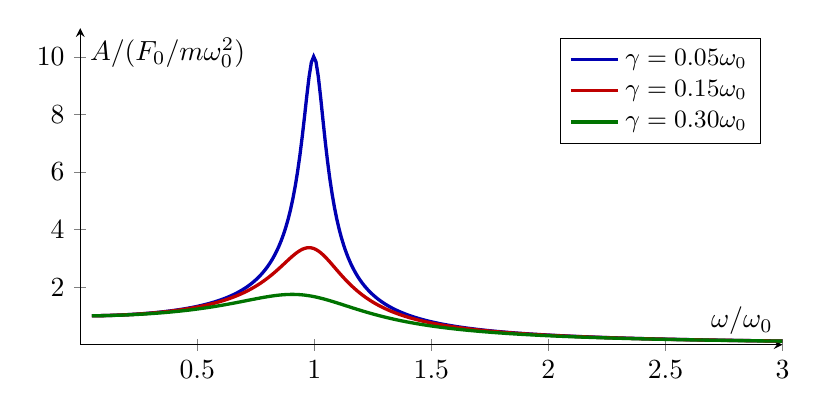
\begin{tikzpicture}
\begin{axis}[
  width=10.5cm,height=5.6cm,
  axis lines=middle,
  xlabel={$\omega/\omega_0$},ylabel={$A/(F_0/m\omega_0^2)$},
  xmin=0,xmax=3,ymin=0,ymax=11,
  xtick={0,0.5,1,1.5,2,2.5,3},
  ytick={0,2,4,6,8,10},
  legend style={at={(0.97,0.97)},anchor=north east,font=\small},
  samples=300,domain=0.05:3
]
\addplot[very thick,blue!70!black] {1/sqrt((1-x^2)^2+4*0.05^2*x^2)};
\addplot[very thick,red!75!black] {1/sqrt((1-x^2)^2+4*0.15^2*x^2)};
\addplot[very thick,green!45!black] {1/sqrt((1-x^2)^2+4*0.3^2*x^2)};
\legend{$\gamma=0.05\omega_0$,$\gamma=0.15\omega_0$,$\gamma=0.30\omega_0$}
\end{axis}
\end{tikzpicture}
\caption{受迫振动的幅频曲线。阻尼越小，共振峰越高、越窄；当 $\omega=\omega_0$ 时相位差为 $\pi/2$。}
\label{fig:resonance}
\end{figure}

\subsection{典型示例}

下面的模型各有不同的受力。先选坐标和正方向，再判断哪些力控制运动。若要从方程求出随时间变化的轨迹，还要写下出发时的位置和速度。

\begin{example}[空间站微重力实验中的受迫振动与三维谐振子]
(1) 在空间站微重力实验平台上，带电粒子（电荷 $-e$）在振荡电场 $E_x=E_0\cos(\omega t+\theta)$ 中运动，$m\ddot x=-eE_x$。积分两次得
\[
x=x_0-\frac{eE_0}{m\omega^2}\cos\theta
+\left(v_0+\frac{eE_0}{m\omega}\sin\theta\right)t
+\frac{eE_0}{m\omega^2}\cos(\omega t+\theta),
\]
即匀速漂移与同频受迫振荡的叠加。

(2) 作为给定外力的教学模型，设三维恢复力可近似为三个独立谐振子（本例不声称仅凭静电场就能形成三维稳定阱）：
\[
m\ddot x_i=-k_i x_i,\qquad x_i=A_i\cos(\omega_i t+\phi_i),\qquad \omega_i=\sqrt{k_i/m}.
\]
对所有被激发的方向，若频率存在共同周期，轨道闭合；若三个频率有理独立，相位轨道在三维相位环面上稠密。仅有某一频率比无理并不足以推出三维环面上的稠密性；位置空间轨迹则是该相位轨道的投影。
\end{example}

\begin{example}[火星探测器进入段的阻力下落模型]
质量为 $m$ 的火星探测器在降落伞展开后的简化模型中，从高度 $h$ 处近似无初速下落，阻力与速度成正比，$\bR=-mk\bv$。取竖直向上为 $x$ 轴正方向，初始位置为 $x(0)=h$，则重力为 $-mg$，阻力为 $-mk\dot x$，运动方程为
\[
m\ddot x=-mg-mk\dot x,
\]
即
\[
\ddot x=-g-k\dot x.
\]
分离变量并积分，利用 $\dot x(0)=0$，
\[
\ln\frac{g+k\dot x}{g}=-kt,
\]
故
\[
\dot x=-\frac{g}{k}\left(1-e^{-kt}\right).
\]
再积分，利用 $x(0)=h$，得
\[
x=h+\frac{g}{k^2}\left(1-e^{-kt}\right)-\frac{g}{k}t.
\]
在形式上的长时间延拓中，$\dot x\to -g/k$，探测器趋于匀速下落，称为\textbf{收尾速度}。若取竖直向下为 $x$ 轴，则速度与坐标的符号整体反转。本模型仅在触地之前使用。线性阻力适用于相应的低雷诺数或经验证的线性范围；实际降落伞及进入段常有速度平方阻力，不能据本例定量预测真实降落过程。

取 $k>0$，将方程写为 $\dd(\dot x+g/k)/\dd t=-k(\dot x+g/k)$。推广到初速 $\dot x(0)=v_0$ 时可得 $\dot x+g/k=(v_0+g/k)e^{-kt}$，再积分一次得到位移。
\end{example}

\begin{example}[月球摆的大振幅周期]
在月球表面，长为 $l$ 的单摆，摆角 $\theta$ 满足
\[
\ddot\theta+\frac{g}{l}\sin\theta=0.
\]
两边乘以 $\dot\theta$ 并积分，得能量积分
\[
\frac12\dot\theta^2-\frac{g}{l}\cos\theta
=\frac12\dot\theta_0^2-\frac{g}{l}\cos\theta_0.
\]
若从最大摆角 $\theta_0$ 处由静止释放，则
\[
\dot\theta^2=\frac{2g}{l}\left(\cos\theta-\cos\theta_0\right).
\]
于是周期为
\[
T=4\sqrt{\frac{l}{g}}\int_0^{\theta_0}
\frac{\dd\theta}{\sqrt{2(\cos\theta-\cos\theta_0)}}.
\]
作 $\sin(\theta/2)=\sin(\theta_0/2)\sin\phi$ 代换，可将它化成第一类完全椭圆积分；章末给出代换细节。小角近似 $\sin\theta\approx\theta$ 给出简谐振动，$T_0=2\pi\sqrt{l/g}$；随着振幅增大，周期变长。按月球平均参数的近似 $g_M\approx1.62\,\mathrm{m/s^2}$，同样长度的摆周期约为地面的 $\sqrt{g/g_M}\approx2.46$ 倍。

\begin{figure}[htbp]
\centering
\begin{tikzpicture}[>=Stealth]
\coordinate (O) at (0,3);\coordinate (B) at (1.2,.921539);
\draw[thick] (-1,3)--(1,3);\draw[thick] (O)--(B);
\draw[dashed] (O)--(0,.5);\fill (B) circle (3pt) node[right]{$m$};
\draw (0,2.1) arc (-90:-60:.9);\node at (.3,1.9) {$\theta$};
\draw[->,thick,red!70!black] (B)--++(0,-.9) node[below]{$m\bg$};
\draw[->,thick,blue!70!black] (B)--++(-.5,.866025) node[left]{$\bT$};
\draw[decorate,decoration={brace,amplitude=4pt}] (.2,3.11547)--(1.4,1.037009) node[midway,right=5pt]{$l$};
\end{tikzpicture}
\caption{固定摆长的单摆：拉力沿绳并垂直瞬时速度，切向重力为 $-mg\sin\theta$。长度标记沿摆线段绘制。}
\label{fig:pendulum}
\end{figure}
\end{example}



\begin{example}[霍尔推进器中的电子]
在霍尔推进器中，电子在互相垂直的均匀电场 $\bE$ 与磁场 $\bB$ 中运动。取 $\bE=E\ii$、$\bB=B\kk$，初速度 $\bv(0)=v_0\jj$，初始位置为原点。求电子的运动规律，并说明漂移速度的物理意义。

\begin{center}
\begin{tikzpicture}[>=Stealth,scale=0.95]
  \draw[->] (0,0)--(4.2,0) node[below]{$x$};
  \draw[->] (0,0)--(0,2.8) node[left]{$y$};
  \draw[->,very thick,red!75!black] (0.6,2.2)--(1.7,2.2) node[above]{$\bE$};
  \node at (0.9,1.25) {$\bB\odot$};
  \draw[->,very thick,green!45!black] (2.8,1.2)--(2.8,2.2) node[right]{$\bv_0$};
  \draw[->,very thick,blue!70!black] (3.5,1.2)--(3.5,0.2) node[right]{$\bv_d=\dfrac{\bE\times\bB}{B^2}$};
\end{tikzpicture}
\end{center}

解：电子电荷为 $-e$，运动方程为
\[
m\dot{\bv}=-e(\bE+\bv\times\bB).
\]
写成分量：
\[
m\dot v_x=-eE-eBv_y,\qquad
m\dot v_y=eBv_x,\qquad
m\dot v_z=0.
\]
令回旋频率 $\omega_c=eB/m$，并定义复速度 $w=v_x+\mathrm{i}v_y$，则
\[
\dot w=-\frac{eE}{m}+\mathrm{i}\omega_c w .
\]
其特解给出漂移速度 $v_x=0$、$v_y=-E/B$，即
\[
\bv_d=\frac{\bE\times\bB}{B^2}.
\]
以初始条件 $w(0)=\mathrm{i}v_0$ 积分，得
\[
v_x(t)=-\left(v_0+\frac{E}{B}\right)\sin\omega_ct,\qquad
v_y(t)=\left(v_0+\frac{E}{B}\right)\cos\omega_ct-\frac{E}{B}.
\]
再积分一次：
\[
x(t)=\frac{v_0+E/B}{\omega_c}(\cos\omega_ct-1),\qquad
y(t)=\frac{v_0+E/B}{\omega_c}\sin\omega_ct-\frac{E}{B}t .
\]
因此电子的运动是“回旋”与“匀速漂移”的叠加：在垂直于 $\bE$ 与 $\bB$ 的方向上，它以速度 $E/B$ 漂移；在以 $\bv_d$ 平动的低速参考系中，它作匀速圆周运动。本模型说明交叉场漂移的单粒子机制。真实霍尔推进器还涉及电离、碰撞及电子输运，离子束电荷中和主要由外置阴极提供电子，不能从这条漂移轨迹直接推出。进一步资料见本章末 NASA 技术介绍。
\end{example}

\section{功、能与势能}

若只想知道滑到底有多快，可以先问各个力在途中做了多少功。这个问题有时比逐时刻求加速度更容易回答。

功和能提供了描述运动的另一套语言：力沿路径的累积效应可以用一个标量——功——来度量，保守力又可以进一步用势能表示。对许多问题，能量守恒比直接求解矢量微分方程更简洁，也更容易揭示运动的全局特征。本节从功的定义出发，引入势能、机械能守恒和势能曲线，为后续的守恒律与中心力问题作准备。

\subsection{功与功率}

拉行李箱时，沿拉力方向移动的那一部分位移决定做功。用同样的力做同样多的功，花的时间越短，平均功率越大。

力 $\bF$ 在微小位移 $\dd\br$ 上做的功为
\begin{equation}
\dd W=\bF\cdot\dd\br=F\cos\alpha\,\dd s,
\end{equation}
其中 $\alpha$ 是力与位移的夹角。这里的 $\dd W$ 表示过程中的元功，一般不是某个仅依赖状态的函数的全微分。沿路径 $L$ 从 $A$ 到 $B$ 的总功为
\begin{equation}
W_{A\to B}=\int_L \bF\cdot\dd\br .
\label{eq:work}
\end{equation}
功率为
\begin{equation}
P=\dv{W}{t}=\bF\cdot\bv .
\end{equation}

\begin{figure}[htbp]
\centering
\begin{tikzpicture}[>=Stealth]
\draw[thick,blue!65!black,domain=-1:2,samples=80] plot (\x,{0.25*\x*\x});
\fill (0,0) circle (2pt) node[below left]{$P$};
\draw[->,very thick,green!40!black] (0,0)--(1.7,0) node[below]{$\dd\br$};
\draw[->,very thick,red!70!black] (0,0)--(1.3,1.3) node[above]{$\bF$};
\draw (0.65,0) arc (0:45:0.65);\node at (0.9,0.3) {$\alpha$};
\end{tikzpicture}
\caption{功只取决于力在瞬时位移上的投影。绿色箭头沿 $P$ 处切线，红色力矢量与它夹角为 $\alpha$。}
\label{fig:work}
\end{figure}

\subsection{保守力与势能}

把书从桌上抬到同一高度，若只算重力的功，走哪条路线结果都相同。这种只由起点和终点决定的功，可以用势能差来记账。

若力沿任意闭合路径做的功为零，
\begin{equation}
\oint_L \bF\cdot\dd\br=0,
\label{eq:conservative-loop}
\end{equation}
则称该力为\textbf{保守力}。等价地，保守力沿 $A\to B$ 的功只与始末位置有关，与路径无关。于是可以定义\textbf{势能} $V(\br)$：
\begin{equation}
V(\br)-V(\br_0)=-\int_{\br_0}^{\br}\bF\cdot\dd\br',
\label{eq:potential}
\end{equation}
或微分形式
\begin{equation}
\bF=-\nabla V .
\label{eq:force-potential}
\end{equation}
在直角坐标中，
\begin{equation}
F_x=-\pdv{V}{x},\qquad F_y=-\pdv{V}{y},\qquad F_z=-\pdv{V}{z}.
\end{equation}
对定义在连通区域内的光滑位置力场，闭路功为零等价于全局单值势能存在。若势能存在，则旋度必为零；反向推论还须区域单连通等拓扑条件。在这样的区域内才可用判据
\begin{equation}
\nabla\times\bF=0
\quad\Longleftrightarrow\quad
\pdv{F_z}{y}=\pdv{F_y}{z},\quad
\pdv{F_x}{z}=\pdv{F_z}{x},\quad
\pdv{F_y}{x}=\pdv{F_x}{y}.
\label{eq:curl-zero}
\end{equation}

\begin{physicsbox}
重力、静电力、弹簧弹力都是保守力；摩擦力、空气阻力一般不是保守力。当势能不显含时间且其余力不做功时，保守力功可由势能变化描述，因此机械能守恒；非保守力的功则把机械能转化为内能等其他形式。
\end{physicsbox}

\subsection{机械能守恒与势能曲线}

把总能量画成水平线，与势能曲线比较。水平线高于势能的区间才可能到达，交点处动能为零；是否真会在交点折返，还要看该处的受力。

质点动能为
\begin{equation}
T=\frac12m\bv^2=\frac12m\dot{\br}^2.
\end{equation}
由牛顿第二定律，
\begin{equation}
\dd T=\bF\cdot\dd\br=\dd W .
\end{equation}
若只有保守力做功，则 $\dd W=-\dd V$，于是
\begin{equation}
\dd(T+V)=0\quad\Longrightarrow\quad T+V=E=\text{常量}.
\label{eq:energy-conservation}
\end{equation}
这就是\textbf{机械能守恒定律}。
更一般地，若 $\bF=-\nabla V(\br,t)+\bF_{\rm nc}$，则
\[
\dot T=-\nabla V\cdot\bv+\bF_{\rm nc}\cdot\bv,\qquad
\dot V=\nabla V\cdot\bv+\pdv{V}{t},
\]
\begin{equation}\label{eq:ch1-energy-general}
\boxed{\frac{\dd}{\dd t}(T+V)=\pdv{V}{t}+\bF_{\rm nc}\cdot\bv.}
\end{equation}
这明确了守恒的条件：时间变化的势或做功的驱动约束都可向质点传递能量。磁力可以不保守却不做功，不能把所有非保守力都等同于耗散力。
\begin{example}[无旋不一定全局保守]
在去掉 $z$ 轴的空间中，取 $\bF=K(-y,x,0)/(x^2+y^2)$，其中 $K$ 的量纲为能量。直接求偏导得到 $\nabla\times\bF=0$。但在半径 $a$ 的圆上，$\br=(a\cos\phi,a\sin\phi,0)$，有 $\bF\cdot\dd\br=K\dd\phi$，故闭路功为 $2\pi K\ne0$。局部可写 $V=-K\phi$，绕轴一周却不单值。这说明使用旋度判据前必须先说明力场定义域。
\end{example}

一维运动的势能曲线 $V(x)$ 提供了运动的定性图像（图中用固定能量与长度单位无量纲化）：由 $E=T+V(x)\ge V(x)$ 可知，运动只能发生在 $V(x)\le E$ 的区间；$V(x)=E$ 的普通单根对应\textbf{转折点}（速度为零并反向）；重根处还可能是平衡或需无限时间才能到达的渐近位置，应单独判断；$V'(x)=0$ 的点为平衡点，$V''(x)>0$ 为稳定平衡，$V''(x)<0$ 为不稳定平衡。若二阶导数为零，须检查更高阶，不能由二阶检验直接定论。

\begin{figure}[htbp]
\centering
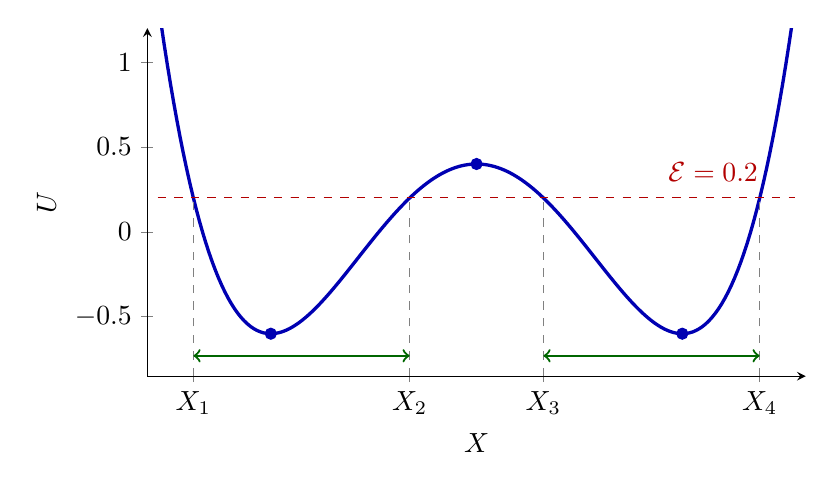
\begin{tikzpicture}
\begin{axis}[width=0.82\textwidth,height=6cm,axis lines=left,
 xlabel={$X$},ylabel={$U$},xmin=-1.6,xmax=1.6,ymin=-.85,ymax=1.2,
 xtick={-1.376382,-.324920,.324920,1.376382},xticklabels={$X_1$,$X_2$,$X_3$,$X_4$}]
\addplot[very thick,blue!70!black,domain=-1.55:1.55,samples=200] {x^4-2*x^2+.4};
\addplot[dashed,red!70!black,domain=-1.55:1.55] {.2};
\addplot[only marks,mark=*,blue!70!black] coordinates {(-1,-.6) (0,.4) (1,-.6)};
\pgfplotsinvokeforeach{-1.376382,-.324920,.324920,1.376382}{\draw[dashed,gray] (axis cs:#1,-.85)--(axis cs:#1,.2);}
\draw[<->,thick,green!40!black] (axis cs:-1.376382,-.73)--(axis cs:-.324920,-.73);
\draw[<->,thick,green!40!black] (axis cs:.324920,-.73)--(axis cs:1.376382,-.73);
\node[red!70!black] at (axis cs:1.15,.35) {$\mathcal E=0.2$};
\end{axis}
\end{tikzpicture}
\caption{无量纲双阱势 $U=X^4-2X^2+0.4$。在能量 $\mathcal E=0.2$ 下，两段绿色区间允许运动，中央势垒不能跨过；四个端点由 $X^2=1\pm\sqrt{0.8}$ 精确确定。}
\label{fig:potential-curve}
\end{figure}

\begin{example}[保守力场的势能]
以下坐标和力按固定长度、力的单位给出数值，势能按相应的力乘长度单位表示。判断 $\bF=(x+2y+z+5)\ii+(2x+y+z)\jj+(x+y+z-6)\kk$ 是否保守，并求势能。

解：三个交叉偏导分别满足 $\partial_yF_x=\partial_xF_y=2$、$\partial_zF_x=\partial_xF_z=1$ 和 $\partial_zF_y=\partial_yF_z=1$。因此在整个 $\mathbb R^3$ 上旋度为零，存在全局势能。先积分 $V_x=-F_x$，得
\[
V=-x^2/2-2xy-xz-5x+g(y,z).
\]
再由 $V_y=-F_y$ 得 $g_y=-y-z$，所以 $g=-y^2/2-yz+h(z)$。最后由 $V_z=-F_z$ 得 $h'=-z+6$。合并得
\[
V=-\left[\frac{x^2}{2}+2xy+xz+5x+\frac{y^2}{2}+yz+\frac{z^2}{2}-6z\right]+C.
\]
取 $V(0,0,0)=0$，则 $C=0$。
\end{example}

\begin{example}[月球车沿抛物线月坑下滑]
月球车（视为质点）质量为 $m$，沿光滑抛物线形月坑 $x^2=4ay$ 从 $x=2a$ 处由静止下滑。求到达坑底时的速度和月面支持力。

解：由 $y=x^2/(4a)$ 得 $y'=x/(2a)$，$y''=1/(2a)$。在 $x=2a$ 处，$y=a$，$y'=1$，切线与水平方向成 $45^\circ$。由机械能守恒，
\[
\frac12mv^2=mg(a-y),
\]
故到达坑底 $y=0$ 时
\[
v=\sqrt{2ga}.
\]
坑底处曲率半径为
\[
\rho=\frac{[1+(y')^2]^{3/2}}{|y''|}\bigg|_{x=0}
=\frac{1}{1/(2a)}=2a.
\]
在坑底，法向（指向曲率中心，即竖直向上）方程为
\[
m\frac{v^2}{\rho}=R-mg.
\]
代入 $v^2=2ga$、$\rho=2a$，得
\[
R=mg+\frac{m(2ga)}{2a}=2mg.
\]
\end{example}
\begin{example}[月球车翻越球形月丘]
月球车（视为质点）质量为 $m$，从半径为 $R$ 的光滑球形月丘顶部附近、极小角位移处由静止释放，并取该位移趋于零的下滑极限。求脱离月丘表面时的位置和速率。

\begin{center}
\begin{tikzpicture}[>=Stealth,scale=1.0]
  \draw[thick] (0,0) circle (1.6);
  \draw[dashed] (0,0)--(0,1.6);
  \coordinate (P) at (1.226,1.028);
  \fill (P) circle (2.2pt) node[above left]{$m$};
  \draw[thick] (0,0)--(P) node[midway,below]{$R$};
  \draw (0,0.7) arc (90:40:0.7);
  \node at (0.22,1.20) {$\theta$};
  \draw[->,thick,red!75!black] (P)--++(0,-0.72) node[below]{$m\bg$};
  \draw[->,thick,blue!70!black] (P)--++(0.52,0.44) node[above right]{$\bN$};
  \draw[->,thick,green!45!black] (P)--++(0.48,-0.40) node[below right]{$\bv$};
\end{tikzpicture}
\end{center}

解：设月球车与竖直方向的夹角为 $\theta$。由机械能守恒，
\[
mgR(1-\cos\theta)=\frac12mv^2 .
\]
沿径向（指向球心）应用牛顿第二定律：
\[
mg\cos\theta-N=m\frac{v^2}{R}.
\]
代入 $v^2=2gR(1-\cos\theta)$，得
\[
N=mg(3\cos\theta-2).
\]
脱离月丘表面的条件是 $N=0$，故
\[
\cos\theta_0=\frac23,\qquad
\theta_0\approx48.2^\circ .
\]
此时速率为
\[
v_0=\sqrt{2gR(1-\cos\theta_0)}
=\sqrt{\frac{2gR}{3}} .
\]
若恰在最高点静止且毫无扰动，它将保持不稳定平衡；上面的下滑结果是微扰极限。在顶部极限 $N=mg$；随着下滑，支持力单调减小，在“赤道”以上就已降为零。此后月球车脱离月丘表面，在月面引力下作弹道运动。
\end{example}


\begin{example}[矩阵力场的势能条件]
设力场由常矩阵 $A=(a_{ij})$ 给出：
\[
\bF=A\br,\qquad F_i=\sum_{j=1}^{3}a_{ij}x_j .
\]
问 $A$ 满足什么条件时 $\bF$ 保守？并求势能。

解：由 $\nabla\times\bF=0$ 得
\[
(\nabla\times\bF)_x=\partial_yF_z-\partial_zF_y=a_{32}-a_{23}=0,
\]
以及其他两个分量循环对称的条件。因此 $\bF$ 保守的充要条件是
\[
a_{ij}=a_{ji},
\]
即 $A$ 为对称矩阵。此时
\[
V(\br)=-\frac12\br^T A\br
=-\frac12\sum_{i,j=1}^{3}a_{ij}x_ix_j
\]
（相差一个常数），且 $-\nabla V=A\br=\bF$。若 $A$ 不对称，只有其对称部分对势能有贡献，反对称部分对应一个不能由势能导出的涡旋力。

把 $A$ 分为对称部分 $S$ 和反对称部分 $W$，有 $\br^{\mathsf T}W\br=0$，因为此标量取转置后反号。逐分量微分给 $\nabla(\br^{\mathsf T}A\br)=(A+A^{\mathsf T})\br$，所以该二次型只能产生 $S\br$。
\end{example}


\section{质点动力学基本定理与守恒定律}

动量、角动量和动能回答不同问题。分别检查外力、绕选定点的外力矩和各力做功，便能知道哪一种量的变化最好算。

\subsection{动量定理与动量守恒}

碰撞力在短时间内可以很大，而且难以逐时刻测定。把力随时间加起来，得到的冲量直接告诉我们动量改变了多少。

由牛顿第二定律 $\bF=\dd\bp/\dd t$，在时间区间 $[t_1,t_2]$ 上积分得
\begin{equation}
\bI=\int_{t_1}^{t_2}\bF\,\dd t=\bp_2-\bp_1,
\label{eq:momentum-theorem}
\end{equation}
其中 $\bI$ 称为\textbf{冲量}。若合外力为零，则
\begin{equation}
\bp=m\bv=\text{常量}.
\label{eq:momentum-conservation}
\end{equation}
这就是\textbf{动量守恒定律}。

\subsection{角动量定理与角动量守恒}

推门时，力的大小相同，推在门把手和推在铰链边的效果不同。选定矩心后，力的大小、方向和力臂共同决定力矩。

质点相对于原点 $O$ 的角动量为
\begin{equation}
\bJ=\br\times\bp=m\,\br\times\bv .
\end{equation}
力矩为
\begin{equation}
\bM=\br\times\bF .
\end{equation}
由
\begin{equation}
\dv{\bJ}{t}=\dv{}{t}(\br\times m\bv)
=\br\times m\ddot{\br}=\br\times\bF=\bM,
\label{eq:angular-momentum-theorem}
\end{equation}
得\textbf{角动量定理}：
\begin{equation}
\dv{\bJ}{t}=\bM .
\end{equation}
若 $\bM=0$，则 $\bJ=\text{常量}$。这里 $O$ 是惯性系中的固定点。若改用移动点 $A(t)$，且角动量仍用绝对动量定义为 $\bJ_A=(\br-\br_A)\times m\bv$，则乘积法则给出
\[
\dot{\bJ}_A=(\bv-\bv_A)\times m\bv+(\br-\br_A)\times\bF
=\bM_A-\bv_A\times\bp.
\]
因此不能不加条件地把固定点角动量定理套到移动参考点。第五章会说明为何质心是一个特别方便的参考点。特别地，若力始终通过某一固定点（中心力），则对该点的角动量守恒。

\begin{physicsbox}
角动量守恒的核心是“力矩为零”，而不是“力为零”。中心力 $\bF=F(r)\er$ 满足 $\br\times\bF=0$，所以角动量守恒；但这并不意味着质点做匀速运动，也不意味着能量一定守恒。
\end{physicsbox}

\subsection{动能定理与守恒律的对称性}

若关心物体快了还是慢了，沿实际位移算功通常最直接。至于动量方向和轨道形状，还要用其他方程或守恒量确定。

由
\begin{equation}
\dd T=m\bv\cdot\dd\bv=\bF\cdot\dd\br=\dd W,
\end{equation}
得\textbf{动能定理}：
\begin{equation}
W_{A\to B}=T_B-T_A=\frac12mv_B^2-\frac12mv_A^2 .
\label{eq:work-energy}
\end{equation}
若只有保守力做功，则 $W=-\Delta V$，从而 $T+V=E$。

进一步看，三个守恒律分别对应时空对称性：空间平移不变 $\Rightarrow$ 动量守恒；空间转动不变 $\Rightarrow$ 角动量守恒；时间平移不变 $\Rightarrow$ 能量守恒。这一对应关系在分析力学中由诺特定理精确表述，是“对称性决定相互作用”的思想源头。

\begin{example}[中心力作用下的平面运动]
质点在中心力 $\bF=F(r)\er$ 作用下运动。由于 $\bM=\br\times\bF=0$，角动量
\[
\bJ=\br\times m\bv
\]
守恒。若 $\bJ\ne0$，因 $\br\cdot\bJ=0$，位矢始终垂直同一个常矢量，轨道位于过力心的固定平面内。若 $\bJ=0$，运动为沿力心直线的径向运动，需单独处理；下式的角度参数化假设 $J\ne0$。

在极坐标中，$\bJ=mr^2\dot\theta\,\kk$，故
\[
mr^2\dot\theta=J=\text{常量}.
\]
扫过的面积速度为
\[
\dv{A}{t}=\frac12r^2\dot\theta=\frac{J}{2m}=\text{常量},
\]
这正是开普勒第二定律的力学基础。
\end{example}

\section{质点系与质心运动}

观察一辆两人推着走的车，可先把人和车合起来研究，再看各部分相对整体怎样运动。系统边界一旦选定，才能分清哪一些力是内力。

本节从每个质点的牛顿第二定律出发，逐步导出质点系的动量、角动量和动能定理。设系统由 $N$ 个质点组成，第 $i$ 个质点的质量为 $m_i$、位矢为 $\br_i$。对每个质点写出牛顿第二定律：
\begin{equation}
m_i\ddot{\br}_i=\bF_i^{(e)}+\sum_{j\ne i}\bF_{ij},
\qquad i=1,\dots,N,
\label{eq:newton-system}
\end{equation}
其中 $\bF_i^{(e)}$ 是外力，$\bF_{ij}$ 是第 $j$ 个质点对第 $i$ 个质点的内力。由牛顿第三定律
\begin{equation}
\bF_{ij}=-\bF_{ji}.
\label{eq:third-law-system}
\end{equation}
以下结论由式 \eqref{eq:newton-system} 和 \eqref{eq:third-law-system} 推出；在讨论内力矩时，还需要假设内力满足强形式。

\subsection{内力、外力与质心}

质心是按质量加权的位置平均。两个人坐跷跷板时，质量较大的一侧对质心位置影响更大，所以平衡时它通常要坐得更靠近支点。

先证明内力之和为零。把内力按 $i<j$ 成对求和：
\begin{equation}
\sum_{i=1}^{N}\sum_{j\ne i}\bF_{ij}
=\sum_{i<j}\left(\bF_{ij}+\bF_{ji}\right)=0.
\label{eq:internal-force-zero}
\end{equation}
若进一步假设内力沿两质点的连线（强形式），则
\begin{equation}
\bF_{ij}\parallel \br_i-\br_j .
\end{equation}
于是每一对内力对固定点 $O$ 的力矩之和为
\begin{equation}
\br_i\times\bF_{ij}+\br_j\times\bF_{ji}
=(\br_i-\br_j)\times\bF_{ij}=0.
\label{eq:internal-torque-zero}
\end{equation}
因此所有内力矩之和也为零。以下各质点质量及系统成员固定；开放系统另行分析。

注意：若内力是运动电荷之间的磁力，强形式一般不成立，必须把电磁场的角动量计入；本节的质点系角动量定理默认内力为中心力。

定义系统的\textbf{质心}
\begin{equation}
\bR=\frac{1}{M}\sum_{i=1}^{N}m_i\br_i,\qquad
M=\sum_{i=1}^{N}m_i .
\label{eq:cm-ch1}
\end{equation}
对连续体，取 $m_i\to\dd m$ 的极限，求和化为积分：
\begin{equation}
\bR=\frac{1}{M}\int\br\,\dd m,\qquad
M=\int\dd m .
\end{equation}
质心不一定在物体上，但它把系统的整体运动浓缩为一个代表点。

\begin{example}[球形贮箱球冠端盖的质心]
航天器中的一个薄壁球形贮箱，被距球心 $b$ 的平面隔板截出一个球冠形端盖（$0<b<a$）。设球面面密度为 $\sigma$，求端盖质心到球心的距离。

\begin{center}
\begin{tikzpicture}[>=Stealth,scale=1.0]
  \fill[blue!8] (0,0) circle (1.5);
  \begin{scope}
    \clip (0,0) circle (1.5);
    \fill[blue!22] (-1.6,0.6) rectangle (1.6,1.6);
  \end{scope}
  \draw[thick,blue!50!black] (0,0) circle (1.5);
  \draw[thick,blue!60!black] (-1.5,0.6)--(1.5,0.6);
  \draw[dashed] (0,0)--(1.5,0) node[midway,below]{$a$};
  \draw[->,thick] (0,0)--(0,2.1) node[above]{$z$};
  \fill (0,1.05) circle (2pt) node[right]{$z_c$};
  \node at (1.0,0.35) {$b$};
  \node at (-1.0,1.15) {球冠端盖};
\end{tikzpicture}
\end{center}

解：设球面面密度为 $\sigma$，取球心为原点、对称轴为 $z$ 轴。球面面积元为
\[
\dd S=2\pi a^2\sin\theta\,\dd\theta,\qquad
z=a\cos\theta,
\]
其中 $\theta$ 从 $0$ 到 $\theta_0$，且 $\cos\theta_0=b/a$。球冠的面积为
\[
S=2\pi a^2\int_0^{\theta_0}\sin\theta\,\dd\theta
=2\pi a(a-b),
\]
质量为 $M=\sigma S$。质心的 $z$ 坐标为
\[
z_c=\frac{1}{S}\int z\,\dd S
=\frac{1}{2\pi a(a-b)}
\int_0^{\theta_0}a\cos\theta\,2\pi a^2\sin\theta\,\dd\theta.
\]
计算积分：
\[
\int_0^{\theta_0}\cos\theta\sin\theta\,\dd\theta
=\frac12\sin^2\theta_0
=\frac12\left(1-\frac{b^2}{a^2}\right).
\]
代入得
\[
z_c=\frac{a^2}{a-b}\cdot\frac12\left(1-\frac{b^2}{a^2}\right)
=\frac{a+b}{2}.
\]
本例忽略端盖厚度且面密度均匀。当 $b=0$ 时，球冠退化为半球面，$z_c=a/2$，这是熟悉的半球壳结果。质心位置直接影响贮箱和航天器的质量特性与姿态控制。
\end{example}

对式 \eqref{eq:cm-ch1} 求导两次，并利用式 \eqref{eq:newton-system}：
\begin{equation}
M\ddot{\bR}
=\sum_i m_i\ddot{\br}_i
=\sum_i\bF_i^{(e)}+\sum_i\sum_{j\ne i}\bF_{ij}.
\end{equation}
由式 \eqref{eq:internal-force-zero}，内力和为零，于是
\begin{equation}
M\ddot{\bR}=\sum_i\bF_i^{(e)}=\bF^{(e)}.
\label{eq:cm-theorem-ch1}
\end{equation}
这就是\textbf{质心运动定理}：质心像一个质量为 $M$、受全部外力矢量和作用的质点。烟花爆炸、航天器分离时，只要外力变化不大，系统质心的轨迹就与爆炸前相同；内部碎片如何飞散不影响质心运动。

\subsection{质点系动量定理与动量守恒}

系统内部互推时，某一部分获得的动量变化会由另一部分抵消。整个系统的动量变化由外界给出的合冲量决定。

由质心定义，系统的总动量为
\begin{equation}
\bP=\sum_i m_i\dot{\br}_i
=\frac{\dd}{\dd t}\sum_i m_i\br_i
=M\dot{\bR}.
\label{eq:system-momentum-def}
\end{equation}
对时间求导，并利用质心运动定理 \eqref{eq:cm-theorem-ch1}：
\begin{equation}
\dv{\bP}{t}=M\ddot{\bR}=\bF^{(e)}.
\label{eq:sys-mom-ch1}
\end{equation}
写成冲量形式：
\begin{equation}
\bP(t_2)-\bP(t_1)=\int_{t_1}^{t_2}\bF^{(e)}\,\dd t .
\end{equation}
若外力和为零，则
\begin{equation}
\bP=M\bV_c=\text{常量}.
\end{equation}
这就是质点系的\textbf{动量守恒定律}。内力可以很大，却不会改变系统的总动量；动量守恒是对整个系统而言的，单个质点的动量一般并不守恒。

\begin{example}[火箭方程]
取竖直向上为正，在所考察高度范围内把 $g$ 近似视为常量。设在 \(\dd t\) 内火箭质量变化为 \(\dd m<0\)，喷出气体相对火箭的速度为 \(-v_e\)（\(v_e>0\)）。喷出前系统动量为 \(mv\)；喷出后火箭动量为 \((m+\dd m)(v+\dd v)\)，气体动量为 \((-\dd m)(v-v_e)\)。外力冲量为 \(-mg\,\dd t\)。由动量定理，
\[
(m+\dd m)(v+\dd v)+(-\dd m)(v-v_e)-mv=-mg\,\dd t .
\]
展开并保留一阶小量：
\[
m\,\dd v+v_e\,\dd m=-mg\,\dd t,
\]
即
\begin{equation}
m\dot v=-v_e\dot m-mg.
\end{equation}
忽略重力时，分离变量并积分：
\begin{equation}
\Delta v=v_e\ln\frac{m_0}{m_f},
\label{eq:rocket-ch1}
\end{equation}
其中 \(m_0,m_f\) 分别为初始质量和燃料耗尽后的质量。若 \(v_e=3.0\,\mathrm{km/s}\)、\(m_0/m_f=10\)，则
\[
\Delta v=3.0\ln10\approx6.9\,\mathrm{km/s}.
\]
质量比越大、排气速度越高，速度增量越大；这就是多级火箭和电推进技术追求高比冲的原因。
\end{example}

\subsection{质点系角动量定理与角动量守恒}

一群物体的总角动量既可以来自整个质心绕外点运动，也可以来自各部分绕质心运动。机器人在自由圆环上爬行时，这两部分都要算。

系统对固定点 $O$ 的总角动量为
\begin{equation}
\bJ=\sum_i\br_i\times m_i\dot{\br}_i .
\end{equation}
对时间求导，并利用式 \eqref{eq:newton-system}：
\begin{equation}
\dv{\bJ}{t}
=\sum_i\br_i\times m_i\ddot{\br}_i
=\sum_i\br_i\times\bF_i^{(e)}
+\sum_i\br_i\times\sum_{j\ne i}\bF_{ij}.
\end{equation}
由式 \eqref{eq:internal-torque-zero}，内力矩成对抵消，于是
\begin{equation}
\dv{\bJ}{t}=\bM^{(e)},\qquad
\bM^{(e)}=\sum_i\br_i\times\bF_i^{(e)}.
\label{eq:sys-ang-ch1}
\end{equation}
若外力对 $O$ 的总力矩为零，则 $\bJ$ 守恒。

为了分离整体转动与内部转动，令
\begin{equation}
\br_i=\bR+\br_i',\qquad
\bv_i=\bV_c+\bv_i'.
\end{equation}
由质心定义，
\begin{equation}
\sum_i m_i\br_i'=0.
\end{equation}
对时间求导得
\begin{equation}
\sum_i m_i\bv_i'=0.
\end{equation}
把 $\br_i,\bv_i$ 代入 $\bJ$：
\begin{equation}
\bJ=\sum_i(\bR+\br_i')\times m_i(\bV_c+\bv_i').
\end{equation}
展开后，含 $\sum m_i\br_i'$ 和 $\sum m_i\bv_i'$ 的交叉项均为零，故
\begin{equation}
\bJ=\bR\times\bP+\bJ',\qquad
\bJ'=\sum_i\br_i'\times m_i\bv_i',
\end{equation}
其中 $\bP=M\bV_c$。第一项是质心的轨道角动量，第二项是系统相对质心的角动量。

\begin{example}[受冲量的双质点杆]
两个质量均为 $m$ 的质点 $A,B$ 由长为 $a$ 的轻杆相连，静止放在光滑水平桌面上。在 $B$ 点施加一个垂直于杆的冲量 $\bI$。求此后质心的速度和杆的角速度。

\begin{center}
\begin{tikzpicture}[>=Stealth,scale=1.0]
  \draw[thick] (0,0)--(4,0);
  \fill (0,0) circle (2.2pt) node[below]{$A$};
  \fill (4,0) circle (2.2pt) node[below]{$B$};
  \fill (2,0) circle (2.2pt) node[below]{$C$};
  \draw[->,very thick,red!75!black] (4,0)--++(0,1.0) node[right]{$\bI$};
  \draw[->,thick,blue!70!black] (2,0)--++(0,0.65) node[right]{$\bV_c$};
  \draw[->] (2.7,0.05) arc (0:120:0.7);
  \node at (3.15,0.55) {$\omega$};
\end{tikzpicture}
\end{center}

解：系统所受外力冲量为 $\bI$，由动量定理
\[
2m\bV_c=\bI\quad\Longrightarrow\quad
\bV_c=\frac{\bI}{2m}.
\]
质心 $C$ 位于杆的中点。对质心的转动惯量为
\[
I_C=2m\left(\frac{a}{2}\right)^2=\frac{ma^2}{2}.
\]
冲量对质心的角冲量为 $(a/2)I$，故
\[
I_C\omega=\frac{a}{2}I
\quad\Longrightarrow\quad
\omega=\frac{I}{ma}.
\]
此后质心以 $\bV_c$ 匀速平动，杆绕质心以 $\omega$ 匀速转动；两质点相对质心的位置矢量作匀速圆周运动。
\end{example}

\begin{example}[自由圆环上的机器人：先找对质心]
细圆环质量 $m$、半径 $R$，质量同为 $m$ 的点状机器人沿环爬行。系统初始静止，无外力及外力矩。令环的转角为 $\varphi$，机器人相对环的角为 $\theta$，其相对环心连线的空间方位为 $\alpha=\varphi+\theta$。机器人相对圆环爬一周时，环转过多少？

解：用 $C$ 表示环心，$G$ 表示总质心。令 $\be(\alpha)$ 为由环心指向机器人的单位矢量，则
\[
\br_b=\br_C+R\be,\quad
\bR_G=\frac{\br_C+\br_b}{2},\quad
\br_C-\bR_G=-\frac R2\be,\quad
\br_b-\bR_G=\frac R2\be.
\]
两者都距总质心 $R/2$，不能把机器人的距质心距离误当作 $R$。关于 $G$ 的角动量是环自转与两部分轨道角动量之和：
\[
J_G=mR^2\dot\varphi+2m(R/2)^2\dot\alpha
=mR^2\left(\dot\varphi+\tfrac12\dot\alpha\right)=0.
\]
因此 $\dd\varphi=-\dd\alpha/2$，又 $\dd\theta=\dd\alpha-\dd\varphi=3\dd\alpha/2$。当 $\Delta\theta=2\pi$ 时，
\[
\boxed{\Delta\alpha=\frac{4\pi}{3},\qquad
\Delta\varphi=-\frac{2\pi}{3}=-120^\circ.}
\]
总质心在空间静止，但环心在动。能量可由机器人内部驱动提供，不能另加“系统动能恒为零”的条件。计算只依赖总爬行角，与具体速度过程无关。
\begin{center}
\begin{tikzpicture}[>=Stealth]
\draw[thick,blue!65!black] (0,0) circle (1.6);
\fill (0,0) circle (2pt) node[below]{$C$};
\fill (0,0.8) circle (2pt) node[right]{$G$};
\fill (0,1.6) circle (3pt) node[above]{机器人};
\draw[<->] (-0.35,0)--(-0.35,0.8) node[midway,left]{$R/2$};
\draw[<->] (-0.35,0.8)--(-0.35,1.6) node[midway,left]{$R/2$};
\draw[->,thick] (1.6,0) arc (0:65:1.6);
\node[right] at (1.7,0.8) {$\alpha=\varphi+\theta$};
\end{tikzpicture}
\end{center}
\end{example}

\subsection{质点系动能定理与柯尼希定理}

向前滚的轮子一边带着质心移动，一边绕质心转。把每个质点的速度分成这两部分后，动能的混合项会因质心定义而消掉。

系统总动能为
\begin{equation}
T=\sum_i\frac12 m_i\dot{\br}_i^2 .
\end{equation}
把 $\dot{\br}_i=\bV_c+\bv_i'$ 代入：
\begin{equation}
T=\frac12\sum_i m_i(\bV_c+\bv_i')^2
=\frac12MV_c^2+\frac12\sum_i m_i v_i'^2
+\bV_c\cdot\sum_i m_i\bv_i'.
\end{equation}
最后一项因 $\sum_i m_i\bv_i'=0$ 而消失，于是
\begin{equation}
T=\frac12MV_c^2+T',\qquad
T'=\sum_i\frac12 m_i v_i'^2 .
\label{eq:koenig-ch1}
\end{equation}
这就是\textbf{柯尼希定理}：总动能等于质心整体运动的动能与相对质心的内部动能之和。

下面从牛顿第二定律导出动能定理。对每个质点，
\begin{equation}
m_i\ddot{\br}_i\cdot\dd\br_i=\bF_i\cdot\dd\br_i,
\end{equation}
对 $i$ 求和：
\begin{equation}
\dd T=\sum_i m_i\ddot{\br}_i\cdot\dd\br_i
=\sum_i\bF_i\cdot\dd\br_i
=\dd W^{(e)}+\dd W^{(i)}.
\label{eq:work-energy-system}
\end{equation}
内力功一般不为零。对一对内力，
\begin{equation}
\dd W_{ij}
=\bF_{ij}\cdot\dd\br_i+\bF_{ji}\cdot\dd\br_j
=\bF_{ij}\cdot\dd(\br_i-\br_j).
\end{equation}
对于定距离的理想中心约束，$\dd(\br_i-\br_j)$ 与 $\br_i-\br_j$ 垂直，而 $\bF_{ij}$ 沿 $\br_i-\br_j$，故内力功为零；对弹簧等系统，内力功则等于对应势能的减少量。

若作用可由不显含时间的总势能描述，可以引入总势能
\begin{equation}
V=\sum_i V_i^{(e)}+\sum_{i<j}V_{ij},
\end{equation}
其中 $V_i^{(e)}$ 是外势能，$V_{ij}$ 是第 $i,j$ 个质点间的相互作用势能。由保守力做功与势能的关系 $\dd W=-\dd V$，结合式 \eqref{eq:work-energy-system} 得
\begin{equation}
\dd(T+V)=0,
\end{equation}
即
\begin{equation}
E=T+V=\text{常量}.
\end{equation}
这就是质点系的\textbf{机械能守恒定律}。

\subsection{两体问题与约化质量}

研究两颗星时，可以先问两星的连线怎样变，再用质心的位置找回各自的位置。约化质量就是把这段相对运动写成一个等效质点所需的质量。

考虑两个质点 $m_1,m_2$，只受彼此的内力作用。由牛顿第二定律，
\begin{equation}
m_1\ddot{\br}_1=\bF_{12},\qquad
m_2\ddot{\br}_2=\bF_{21},\qquad
\bF_{21}=-\bF_{12}.
\end{equation}
定义相对位矢和质心
\begin{equation}
\br=\br_1-\br_2,\qquad
\bR=\frac{m_1\br_1+m_2\br_2}{m_1+m_2}.
\end{equation}
两式相减：
\begin{equation}
\ddot{\br}=\ddot{\br}_1-\ddot{\br}_2
=\frac{\bF_{12}}{m_1}-\frac{\bF_{21}}{m_2}
=\left(\frac1{m_1}+\frac1{m_2}\right)\bF_{12}.
\end{equation}
定义约化质量
\begin{equation}
\mu=\frac{m_1m_2}{m_1+m_2},
\end{equation}
则
\begin{equation}
\mu\ddot{\br}=\bF_{12}.
\label{eq:reduced-ch1}
\end{equation}
同时，
\begin{equation}
(m_1+m_2)\ddot{\bR}
=m_1\ddot{\br}_1+m_2\ddot{\br}_2
=\bF_{12}+\bF_{21}=0,
\end{equation}
所以质心作匀速直线运动。若两体内力进一步仅依赖相对距离且沿连线，两体问题因此化为一个质量为 \(\mu\) 的质点在中心力 \(\bF_{12}\) 中的单体问题；相对运动的具体轨道可直接引用后续中心力部分的结果，无需重新推导开普勒定律。

相对坐标与质心坐标还能反解原位置：
\[
\br_1=\bR+\frac{m_2}{m_1+m_2}\br,\qquad
\br_2=\bR-\frac{m_1}{m_1+m_2}\br.
\]
微分后代入总动能，交叉项因 $m_1m_2/(m_1+m_2)-m_2m_1/(m_1+m_2)=0$ 抵消，剩下
\begin{equation}\label{eq:ch1-twobody-energy}
T=\tfrac12(m_1+m_2)\dot{\bR}^{\,2}+\tfrac12\mu\dot{\br}^{\,2},\qquad
\bJ_G=\br\times\mu\dot{\br}.
\end{equation}
若势能为 $V(r)$，相对能量 $E_{\rm rel}=\mu\dot{\br}^{\,2}/2+V(r)$ 独立守恒；不能把一个粒子相对地面的速度直接当作相对速度。

\begin{example}[双星系统的动能]
两颗星质量分别为 $m_1,m_2$，相距 $r$，绕共同质心作匀速圆周运动。求系统的总动能。

\begin{center}
\begin{tikzpicture}[>=Stealth,scale=1.0]
  \fill (0,0) circle (3pt) node[below]{$m_1$};
  \fill (4,0) circle (2pt) node[below]{$m_2$};
  \fill (1.3,0) circle (2pt) node[below]{$C$};
  \draw[dashed] (0,0)--(4,0) node[midway,above]{$r$};
  \draw[->,thick,blue!70!black] (0,0)--++(0,0.8) node[left]{$\bv_1$};
  \draw[->,thick,red!75!black] (4,0)--++(0,-0.65) node[right]{$\bv_2$};
\end{tikzpicture}
\end{center}

解：质心静止，故由柯尼希定理 $T=T'$。相对运动满足式 \eqref{eq:reduced-ch1}。由动量守恒 $m_1v_1=m_2v_2$，且 $v=v_1+v_2$，可解出
\[
v_1=\frac{m_2}{m_1+m_2}v,\qquad
v_2=\frac{m_1}{m_1+m_2}v .
\]
相对运动是半径为 $r$ 的圆周运动，向心加速度为 $v^2/r$，引力大小为 $Gm_1m_2/r^2$，故
\[
\frac{m_1m_2}{m_1+m_2}\frac{v^2}{r}
=\frac{Gm_1m_2}{r^2},
\]
即 $v^2=G(m_1+m_2)/r$。代入动能：
\[
T=\frac12m_1v_1^2+\frac12m_2v_2^2
=\frac12\frac{m_1m_2}{m_1+m_2}v^2
=\frac{Gm_1m_2}{2r}.
\]
这个结果也可以看作“约化质量 $\mu$ 的动能”。
\end{example}

\begin{example}[空间站释放立方星：质心系中的反冲]
空间站质量为 $M$，一颗立方星质量为 $m$，二者由压缩弹簧连接，初始相对静止。弹簧释放能量 $E_s$ 后把立方星推出。忽略轨道曲率、潮汐力和空气阻力，求二者相对速度、各自速度，并说明质心运动。

\begin{center}
\begin{tikzpicture}[>=Stealth,scale=1.0]
  \draw[thick,fill=gray!15] (0,0.2) rectangle (2.2,1.0);
  \node at (1.1,1.2) {空间站 $M$};
  \fill (1.1,0.5) circle (2pt) node[below]{$C$};
  \draw[decorate,decoration={coil,amplitude=3pt,segment length=4pt}]
    (2.3,0.35)--(3.3,0.35);
  \node[above] at (2.8,0.55) {弹簧};
  \fill[fill=gray!45] (3.5,0.15) rectangle (3.9,0.75);
  \node at (3.7,-0.15) {$m$};
  \draw[->,thick,blue!70!black] (1.1,0.5)--++(-0.8,0) node[left]{$V$};
  \draw[->,thick,red!75!black] (3.9,0.5)--++(0.8,0) node[right]{$v$};
\end{tikzpicture}
\end{center}

解：在质心系中，系统总动量为零。设空间站和立方星的速度分别为 $V$ 和 $v$，方向相反，则
\[
MV+mv=0.
\]
设二者分离的相对速度为 $u=v-V$，解得
\[
v=\frac{M}{M+m}u,\qquad
V=-\frac{m}{M+m}u.
\]
弹簧释放的能量全部转化为质心系中的动能：
\[
E_s=\frac12MV^2+\frac12mv^2
=\frac12\frac{Mm}{M+m}u^2
=\frac12\mu u^2,
\]
其中 $\mu=Mm/(M+m)$ 为约化质量。因此
\[
u=\sqrt{\frac{2E_s}{\mu}},\qquad
v=\frac{M}{M+m}u,\qquad
V=-\frac{m}{M+m}u.
\]
质心不受额外外力，继续沿原轨道运动；释放过程只改变系统内部相对运动，不改变质心轨道。以下是教学设定，不是空间站实测数据。若取 $M=4.2\times10^5\,\mathrm{kg}$、$m=10\,\mathrm{kg}$、$E_s=10\,\mathrm{J}$，则
\[
u\approx1.4\,\mathrm{m/s},\qquad
|V|\approx3.4\times10^{-5}\,\mathrm{m/s}.
\]
空间站的反冲速度极小，而立方星获得约 $1.4\,\mathrm{m/s}$ 的分离速度。这里“质心不动”仅指所选质心系；在地心惯性系中质心仍运动。短时忽略潮汐的条件下，可把它近似为沿原轨道运动。
\end{example}

\begin{example}[地月系统的质心]
地球质量 \(M_E\approx5.97\times10^{24}\,\mathrm{kg}\)，月球质量 \(M_m\approx7.35\times10^{22}\,\mathrm{kg}\)，地月距离 \(d\approx3.84\times10^8\,\mathrm{m}\)。约化质量为
\[
\mu=\frac{M_EM_m}{M_E+M_m}\approx7.25\times10^{22}\,\mathrm{kg}.
\]
质心到地心的距离为
\[
d_E=\frac{M_m}{M_E+M_m}d\approx4.67\times10^6\,\mathrm{m},
\]
小于地球平均半径（约 $6.37\times10^6\,\mathrm{m}$），所以地月质心位于地球内部。严格说，地球和月球都绕这个共同质心运动；把月球看作绕静止地球只是近似。
\end{example}

\subsection{碰撞：质心系为什么能简化计算？}\label{sec:newton-collision}
两辆小车相撞，先减去它们共同的质心速度，就只剩相向接近或彼此分离的运动。恢复系数比较的正是接近和分离的相对速率。

碰撞时间很短，若外力冲量相对接触冲量可忽略，则总动量在碰撞前后近似守恒。不应把这一近似写成“碰撞时外力一定为零”。考虑一维正碰，初速度为 $u_1,u_2$，末速度为 $v_1,v_2$，取 $u_1-u_2>0$ 表示接近。质心速度
\[
V_G=\frac{m_1u_1+m_2u_2}{m_1+m_2}
=\frac{m_1v_1+m_2v_2}{m_1+m_2}
\]
在碰撞中不变。高速碰撞见第\ref{sec:sr-collision}节。用恢复系数描述分离相对速度：
\[
v_1-v_2=-e_r(u_1-u_2),\qquad 0\le e_r\le1.
\]
令 $w=u_1-u_2$，解动量及相对速度两式可得
\begin{align}
v_1&=V_G-\frac{m_2}{m_1+m_2}e_rw,\\
v_2&=V_G+\frac{m_1}{m_1+m_2}e_rw.
\end{align}
由式 \eqref{eq:ch1-twobody-energy}，质心平动能不变，损失的动能只来自相对运动：
\begin{equation}\label{eq:ch1-collision-loss}
T_{\rm before}-T_{\rm after}=\tfrac12\mu(1-e_r^2)w^2.
\end{equation}
完全弹性碰撞 $e_r=1$ 保持总动能；完全非弹性正碰 $e_r=0$ 时两物体同速。耗散的动能可变成形变和内能，总能量仍守恒。该单一恢复系数模型不包括斜碰中的摩擦和转动。
\begin{example}[一维碰撞的极限检查]
质量 $m$ 的粒子以速度 $u>0$ 撞上静止靶 $M$，取 $e_r=1$。上式给出
\[
v_1=\frac{m-M}{m+M}u,\qquad
v_2=\frac{2m}{m+M}u.
\]
若 $m=M$，二者交换速度；若 $M\gg m$，入射粒子近似以 $-u$ 反弹，而靶速度很小。若改取 $e_r=0$，共同速度为 $mu/(m+M)$，动能损失为 $mMu^2/[2(m+M)]$。质量相等且靶静止时，完全结合损失初始动能的一半，不能同时再要求动能守恒。

取 $m$ 为入射质量、$M$ 为静止靶。解 $mv_1+Mv_2=mu$、$v_2-v_1=e_ru$ 得 $v_1=(m-e_rM)u/(m+M)$、$v_2=(1+e_r)mu/(m+M)$。损失可直接用质心系动能 $\frac12[mM/(m+M)](v_2-v_1)^2$ 与碰前相对动能比较。
\end{example}
\begin{physicsbox}[title={物理图像与理解：把共同平移从碰撞中拿走}]
实验室看到两物体既共同前进又相互接近，容易混淆这两部分运动。在质心系中，二者动量大小相等、方向相反；一维弹性碰撞只将它们反向。解完内部碰撞再加回同一个 $V_G$，即可返回实验室系。质心系是惯性系的前提是该阶段合外力为零或可忽略。
\end{physicsbox}
\begin{figure}[htbp]
\centering
\begin{tikzpicture}[>=Stealth]
\node[anchor=west] at (-1.1,1.2) {碰前};
\node[anchor=west] at (-1.1,-0.2) {碰后};
\foreach \y in {1.2,-0.2}{
\fill[blue!70!black] (1,\y) circle (3pt);
\fill[red!70!black] (4,\y) circle (4pt);}
\draw[->,thick,blue!70!black] (1,1.2)--(2,1.2) node[midway,above]{$+p_*$};
\draw[->,thick,red!70!black] (4,1.2)--(3,1.2) node[midway,above]{$-p_*$};
\draw[->,thick,blue!70!black] (1,-0.2)--(0,-0.2) node[midway,below]{$-p_*$};
\draw[->,thick,red!70!black] (4,-0.2)--(5,-0.2) node[midway,below]{$+p_*$};
\end{tikzpicture}
\caption{质心系中的一维弹性碰撞。箭头表示动量，各物体速度还须分别除以自身质量；两物体的动量相消，但动能不为零。}
\label{fig:ch1-cm-collision}
\end{figure}

\subsection{位力定理}

物体绕行一周时，动能和势能可以一直变化，但它们的长时间平均可能有简单关系。这里的关键是区分有界运动的平均与某个时刻的瞬时值。

定义位力
\begin{equation}
G=\sum_i\bp_i\cdot\br_i .
\end{equation}
利用 \(\dot{\bp}_i=\bF_i\) 和 \(\bp_i=m_i\dot{\br}_i\)，对时间求导：
\begin{equation}
\dot G=\sum_i\dot{\bp}_i\cdot\br_i+\sum_i\bp_i\cdot\dot{\br}_i
=\sum_i\bF_i\cdot\br_i+2T .
\end{equation}
对时长 $\mathcal T$ 取平均，严格有
\[
\frac{G(t_0+\mathcal T)-G(t_0)}{\mathcal T}
=2\langle T\rangle_{\mathcal T}
+\left\langle\sum_i\bF_i\cdot\br_i\right\rangle_{\mathcal T}.
\]
只有当左边在 $\mathcal T\to\infty$ 时趋零，且右边平均存在，才得到\textbf{位力定理}
\begin{equation}
2\langle T\rangle+\left\langle\sum_i\bF_i\cdot\br_i\right\rangle=0.
\label{eq:virial-ch1}
\end{equation}
$G$ 有界是充分条件，位置有界本身并不自动保证动量有界，特别是存在碰撞奇点时。周期运动可直接取整数周期平均。

若全部力来自不显含时间的 $n$ 次齐次势 $V$，欧拉齐次函数定理给出
\[
\sum_i\br_i\cdot\nabla_iV=nV,\qquad 2\langle T\rangle=n\langle V\rangle.
\]
平方反比引力的势能次数为 $-1$，故 $2\langle T\rangle+\langle V\rangle=0$。对引力系统应使用质心内部动能，否则整体平动会污染估计。
\begin{modernbox}[title={进一步探索：位力质量估计的假设}]
若用模型 $V\simeq-CGM^2/R$，其中 $C$ 依赖密度分布，并定义三维内部均方速度 $\langle v^2\rangle$，则 $T=M\langle v^2\rangle/2$，估计为 $M\simeq R\langle v^2\rangle/(CG)$。若观测量是一维视向速度弥散 $\sigma_{\rm los}$，还需各向同性等假设才有 $\langle v^2\rangle=3\sigma_{\rm los}^2$。因此没有不注明速度定义与结构系数的通用质量公式。进一步学习需统计平均与引力势能积分，可先用均匀球完成章末习题。
\end{modernbox}

\section{非惯性参考系}

公交车突然起步时，乘客在车内看起来向后偏。若坚持在车里写方程，就要把车本身的加速带来的影响一起算进去。

前面讨论的参考系都默认是惯性系。实际观测中，我们常常身处加速或转动的参考系，例如加速的车厢、旋转的地球和太空电梯。只要在牛顿第二定律中引入相应的惯性力，非惯性系中的运动方程仍可写成“合力等于质量乘加速度”的形式。本节先建立相对运动的普遍关系，再讨论平动、转动参考系中的惯性力，并以地球自转和太空电梯为例说明其物理效应。

\subsection{相对运动与伽利略变换}

当两位观察者彼此匀速移动时，从一人的位置读数中减去另一坐标原点的运动，就能得到新读数。再微分一次得速度关系，两次得加速度关系。

设有两个参考系 $S$ 与 $S'$。$S'$ 的原点 $O'$ 在 $S$ 中的位矢为 $\bR(t)$。同一质点 $P$ 在 $S$ 中的位矢为 $\br$，在 $S'$ 中的位矢为 $\br'$，则
\begin{equation}
\br=\bR+\br'.
\label{eq:relative-position}
\end{equation}
对时间求导：
\begin{equation}
\bv=\dot{\bR}+\bv',\qquad
\ba=\ddot{\bR}+\ba'.
\label{eq:relative-velocity}
\end{equation}
若 $S'$ 相对 $S$ 作匀速直线平动，则 $\ddot{\bR}=0$，于是 $\ba=\ba'$。这说明加速度在相互作匀速直线平动的参考系中相同，为伽利略相对性原理的运动学基础。

\begin{figure}[htbp]
\centering
\begin{tikzpicture}[>=Stealth,scale=1.05]
  \draw[->] (0,0)--(5.2,0) node[below]{$x$};
  \draw[->] (0,0)--(0,3.5) node[left]{$y$};
  \coordinate (O) at (0,0);
  \coordinate (Op) at (1.8,0.75);
  \coordinate (P) at (4.0,2.7);
  \draw[->,very thick,blue!65!black] (O)--(Op) node[midway,below]{$\bR$};
  \draw[->] (Op)--++(2.6,0) node[below]{$x'$};
  \draw[->] (Op)--++(0,2.2) node[left]{$y'$};
  \draw[->,very thick,red!75!black] (O)--(P) node[pos=0.55,above left]{$\br$};
  \draw[->,very thick,green!45!black] (Op)--(P) node[midway,right]{$\br'$};
  \fill (P) circle (1.7pt) node[above right]{$P$};
  \node at (0.5,0.3) {$S$};
  \node at (2.2,1.4) {$S'$};
\end{tikzpicture}
\caption{两个参考系中的位矢关系 $\br=\bR+\br'$。若 $S'$ 相对 $S$ 平动，则三个矢量构成一个随时间变化的三角形。}
\label{fig:frames}
\end{figure}

最重要的特殊情形是伽利略变换。若 $S'$ 相对 $S$ 以恒定速度 $\bV$ 沿 $x$ 轴平动，且 $t=0$ 时两原点重合，则
\begin{equation}
x'=x-Vt,\qquad y'=y,\qquad z'=z,\qquad t'=t.
\label{eq:galilean}
\end{equation}
这是对同一事件换用运动参考系坐标的被动变换。第\ref{ch:relativity}章式 \eqref{eq:sr-lorentz} 在低速且同时性修正可忽略时恢复此式。
对时间求导得
\begin{equation}
v_x'=v_x-V,\qquad v_y'=v_y,\qquad v_z'=v_z,
\end{equation}
再求导得
\begin{equation}
a_x'=a_x,\qquad a_y'=a_y,\qquad a_z'=a_z .
\end{equation}
因此，在伽利略变换下加速度不变，牛顿第二定律的形式也不变。这就是\textbf{伽利略相对性原理}：一切惯性系对力学规律等价，不存在“绝对静止”的惯性系。

\begin{modernbox}
伽利略变换隐含了绝对时间 $t'=t$ 和绝对空间（长度不变）的假设。狭义相对论表明，当速度接近光速时，这些假设失效，应由洛伦兹变换替代。但在 $v\ll c$ 的经典力学范围内，伽利略变换是极好的近似。本书前六章除特别说明外均采用经典时空观。
\end{modernbox}

\begin{example}[理想径向收绳：角动量如何限制回收过程？]
在惯性平面内，一载荷以质量 $m$ 的质点建模，轻绳另一端固定于原点。绳始终绷紧，张力沿径向；卷扬机规定 $\dot r=-u$，$u>0$，初始 $r=r_0$，比角动量为 $h>0$。忽略其他力，求可行收绳阶段的轨道与张力。

解：力矩为零，故 $r^2\dot\theta=h$。而 $r=r_0-ut$，因此
\[
\theta(t)-\theta_0=\int_0^t\frac{h\,\dd t'}{(r_0-ut')^2}
=\frac hu\left(\frac1{r(t)}-\frac1{r_0}\right).
\]
由 $m(\ddot r-r\dot\theta^2)=-T$ 且 $\ddot r=0$ 得
\[
T=\frac{mh^2}{r^3},\qquad
\frac{\dd}{\dd t}\left[\frac m2(u^2+h^2/r^2)\right]
=\frac{mh^2u}{r^3}=Tu.
\]
收绳机构对载荷做正功，横向速率随 $r$ 减小而增大。模型形式上在 $r\to0$ 时要求无限张力与能量；实际必须在有限捕获半径停止、减速或转移动量。不存在只比较“横向速度与收绳速度”就能判断捕获的普遍准则；本题也不描述空间站轨道系中的完整相对动力学。
\end{example}



\subsection{加速平动参考系}

在向上加速的电梯里，人会感觉更重。把地面系中的加速度改写为相对于电梯的加速度，就能看出为什么电梯里出现一个额外的向下项。

设惯性系 $S$ 中质点受力 $\bF$，加速度为 $\ba$。另一参考系 $S'$ 相对 $S$ 以加速度 $\ba_0$ 平动，则质点在 $S'$ 中的加速度为
\[
\ba'=\ba-\ba_0.
\]
代入牛顿第二定律，
\begin{equation}
m\ba'=\bF-m\ba_0 .
\label{eq:accel-frame}
\end{equation}
若把 $-m\ba_0$ 称为\textbf{惯性力}，则形式上仍有“合力 = 质量 $\times$ 加速度”。惯性力不是物体间的相互作用，没有反作用力，只在非惯性系中出现。

\begin{physicsbox}
在加速的车厢中，乘客感到一个向后的“力”，这就是惯性力。它可以局域地等效于引力场：$-\,m\ba_0$ 与 $m\bg$（均匀引力）在动力学上不可区分。这一观察是爱因斯坦等效原理的起点。
\end{physicsbox}

\subsection{转动参考系}

坐标轴一旦转动，速度箭头即使相对这些轴分量不变，在地面看也可能转向。对转动基矢求导，正是各个附加项的来源。

设 $S'$ 相对惯性系 $S$ 以角速度 $\bom$ 转动，且两原点重合。取 $S'$ 的基矢量为 $\be_i'$，则基矢量随 $S'$ 转动：
\begin{equation}
\dv{\be_i'}{t}=\bom\times\be_i'.
\end{equation}
把任意矢量写成 $\bA=A_i'\be_i'$，在惯性系 $S$ 中求导：
\begin{equation}
\left(\dv{\bA}{t}\right)_S
=\dot A_i'\be_i'+A_i'\dot{\be}_i'
=\left(\dv{\bA}{t}\right)_{S'}+\bom\times\bA .
\label{eq:rotating-derivative}
\end{equation}
第一项是 $S'$ 中观察到的变化率，第二项来自基矢量的转动。

取 $\bA=\br$，得速度关系
\begin{equation}
\bv=\bv'+\bom\times\br .
\label{eq:rotating-velocity}
\end{equation}
再对 $\bv$ 应用式 \eqref{eq:rotating-derivative}：
\begin{align}
\ba&=\left(\dv{\bv}{t}\right)_S
=\left(\dv{\bv}{t}\right)_{S'}+\bom\times\bv \nonumber\\
&=\ba'+\dot{\bom}\times\br+\bom\times\bv'
+\bom\times(\bv'+\bom\times\br)\nonumber\\
&=\ba'+2\bom\times\bv'+\bom\times(\bom\times\br)
+\dot{\bom}\times\br .
\label{eq:rotating-acceleration}
\end{align}
代入牛顿第二定律，得到转动系中的运动方程
\begin{equation}
m\ba'=\bF
-2m\bom\times\bv'
-m\bom\times(\bom\times\br)
-m\dot{\bom}\times\br .
\label{eq:rotating-eom}
\end{equation}
后三项对应的惯性力依次为：
\begin{itemize}[leftmargin=2.2em]
  \item \textbf{科里奥利力} $\bF_C=-2m\bom\times\bv'$；
  \item \textbf{离心力} $\bF_{\rm cf}=-m\bom\times(\bom\times\br)$，当 $\bom\perp\br$ 时大小为 $m\omega^2\rho$，方向背离转轴；
  \item \textbf{欧拉力} $\bF_E=-m\dot{\bom}\times\br$，只在角速度变化时出现。
\end{itemize}

\begin{figure}[htbp]
\centering
\begin{tikzpicture}[>=Stealth]
\begin{scope}
\draw[thick,fill=gray!8] (0,0) rectangle (3,2);
\fill (1.5,1) circle (3pt) node[above]{$m$};
\draw[->,thick,blue!70!black] (1.5,1)--(.3,1) node[midway,below]{$-m\ba_0$};
\draw[->,thick] (1.8,2.3)--(3,2.3) node[right]{$\ba_0$};
\node at (1.5,-.6) {(a) 加速平动系};
\end{scope}
\begin{scope}[shift={(6,0)}]
\draw[->] (0,0)--(3.6,0) node[right]{$x'$};\draw[->] (0,-1.2)--(0,2.5) node[above]{$y'$};
\node[left] at (0,0) {$O$};\node at (.7,2.2) {$\bom\odot$};
\coordinate (P) at (2,0);\fill (P) circle (3pt);
\draw[->,thick,red!70!black] (P)--(2,1.2) node[above]{$\bv'$};
\draw[->,thick,green!40!black] (P)--(3.2,0) node[above]{$\bF_C$};
\draw[->,thick,blue!70!black] (2,-.45)--(3.2,-.45) node[below]{$\bF_{\rm cf}$};
\node at (1.6,-1.6) {(b) 在 $+x'$ 轴的粒子};
\end{scope}
\end{tikzpicture}
\caption{明确取 $\bom$ 垂直纸面向外。(b) 粒子位于 $+x'$ 轴且相对速度沿 $+y'$，于是 $-2m\bom\times\bv'$ 和离心力都沿 $+x'$；离心力箭头为便于辨认平移绘出。}
\label{fig:noninertial}
\end{figure}

\subsection{地球自转效应}

地面实验室随地球一起转。分析落体或摆时，先按东、北、竖直分解地球角速度，再判断哪些转动效应在题目的精度下需要保留。

在地球表面，取随地球转动的参考系。地球自转角速度记为 $\omega$。把 $\bom$ 分解为当地竖直分量和水平分量：
\begin{equation}
\bom=\omega\left(\cos\lambda\,\hat{\boldsymbol{\jmath}}_{\rm north}
+\sin\lambda\,\hat{\boldsymbol{k}}_{\rm up}\right),
\end{equation}
其中 $\lambda$ 为地理纬度。科里奥利力
\begin{equation}
\bF_C=-2m\bom\times\bv'
\end{equation}
对纯水平速度，科里奥利力的水平分量大小为
\begin{equation}
|F_{C,\rm horizontal}|=2m\omega v|\sin\lambda|,
\end{equation}
对纯水平运动，它使物体在北半球向右偏、南半球向左偏。其中 $\lambda$ 为地理纬度。

对傅科摆的小幅摆动，设摆锤在水平面内的坐标为 $(x,y)$，则科里奥利加速度的水平分量为 $(2\omega\sin\lambda\,\dot y,-2\omega\sin\lambda\,\dot x)$。于是
\begin{equation}
\ddot x-2\omega\sin\lambda\,\dot y+\omega_0^2x=0,\qquad
\ddot y+2\omega\sin\lambda\,\dot x+\omega_0^2y=0,
\end{equation}
其中 $\omega_0=\sqrt{g/l}$。这组方程的解表明，摆动平面以角速度 $\omega\sin\lambda$ 缓慢进动，进动周期为
\begin{equation}
T_{\rm F}=\frac{2\pi}{\omega|\sin\lambda|}.
\end{equation}
此处 $g$ 已吸收当地静态离心修正，忽略 $\omega^2$ 的其他影响；周期分子是恒星日，而非严格的24小时。赤道处该阶进动为零，周期趋于无穷；进动方向在两半球相反。

\begin{modernbox}
大尺度大气运动和长程弹道需要评估地球自转项。判断是否可以忽略科里奥利效应，可比较特征速度 $U$、长度 $L$ 与转速，构造罗斯贝数 $\mathrm{Ro}=U/(2\omega L)$。局部小尺度运动不能只凭“位于北半球”就断言自转项占主导。
\end{modernbox}

\begin{example}[绕竖直直径旋转的圆环与小珠]
在地面实验舱中，半径为 $R$ 的光滑圆形导轨以恒定角速度 $\omega$ 绕竖直直径转动，研究离心效应与重力竞争；小环质量为 $m$，套在导轨上。以最低点为 $\theta=0$，转动系中的有效势能为
\[
V_{\rm eff}(\theta)=-mgR\cos\theta-\frac12m\omega^2R^2\sin^2\theta.
\]
平衡条件 $V_{\rm eff}'=0$ 给出
\[
\sin\theta\left(g-\omega^2R\cos\theta\right)=0.
\]
故平衡位置为 $\theta=0,\pi$，以及（当 $\omega^2>g/R$ 时，左右各有一个对称位置）
\[
\cos\theta_0=\frac{g}{\omega^2R}.
\]
$\theta=0$ 在 $\omega^2<g/R$ 时稳定，在 $\omega^2>g/R$ 时失稳；$\theta=\pi$ 恒不稳定；$\theta_0$ 稳定。这是离心力导致的\emph{分岔}：转速增大到临界值时，最低点失稳，系统转向新的稳定平衡。本例假定地面均匀重力。失重旋转舱应取相应的微重力模型，不能直接照搬地面平衡角。

由 $V_{\rm eff}''=mR[g\cos\theta-\omega^2R\cos(2\theta)]$，最低点和最高点的曲率分别为 $mR(g-\omega^2R)$ 和 $-mR(g+\omega^2R)$，新平衡支的曲率为 $m\omega^2R^2\sin^2\theta_0$。恰在临界转速，原点的二次项消失，而 $V_{\rm eff}(\theta)-V_{\rm eff}(0)=\frac{mgR}{2}(1-\cos\theta)^2$，最低点仍是严格局部极小，恢复力的首项为三阶。
\end{example}

\begin{figure}[htbp]
\centering
\begin{tikzpicture}[>=Stealth,scale=1.0]
  \draw[thick] (0,3.3)--(0,-0.3);
  \draw[blue!45,thick] (0,1.5) circle (1.5);
  \draw[dashed] (0,1.5)--(0,3.0);
  \fill (1.06,0.44) circle (2.4pt) node[below right]{$m$};
  \draw[->,thick,red!75!black] (1.06,0.44)--++(0,-0.9) node[below]{$m\boldsymbol g$};
  \draw[->,thick,blue!70!black] (1.06,0.44)--++(1.0,0) node[above right]{$m\omega^2\rho$};
  \draw[->,thick,green!45!black] (1.06,0.44)--++(-0.65,0.65) node[midway,below left]{$\bN$};
  \draw (0,1.5)--(1.06,0.44);
  \draw (0,1.5) ++(-90:0.75) arc (-90:-40:0.75);
  \node at (0.30,0.95) {$\theta$};
  \draw[->] (1.75,2.9) arc (60:20:1.0);
  \node at (2.25,2.75) {$\omega$};
\end{tikzpicture}
\caption{绕竖直直径旋转的圆环与小珠。转动系中，重力、约束力与离心力共同决定平衡位置；当 $\omega^2>g/R$ 时，最低点失稳，出现偏离竖直方向的稳定平衡。}
\label{fig:rotating-hoop}
\end{figure}


\subsection{太空电梯：旋转系中的有效引力}

沿赤道上方的旋转缆绳移动时，引力随高度减弱，而随地球转动所需的向心加速度随半径增大。比较两者就能判断不同高度处缆绳怎样受拉。

太空电梯的设想是：从地球赤道向外延伸一根缆绳，顶端系一个配重，使整根缆绳随地球自转。缆绳上的每一点都在旋转系中静止，因此可以直接用离心力与引力的平衡来分析。这个例子把非惯性系、有效势能和材料强度联系起来，是现代空间工程中的经典力学问题。

\begin{example}[太空电梯的张力与视重]
设地球质量为 $M$、半径为 $R_E$、自转角速度为 $\Omega$。缆绳沿赤道径向向外，线密度为 $\mu$，顶端 $r_t$ 处连接配重。求缆绳中的张力分布、同步轨道半径，以及攀爬器在缆绳上的视重和科里奥利偏转。

\begin{center}
\begin{tikzpicture}[>=Stealth,scale=0.9]
  \shade[ball color=blue!20] (0,0) circle (0.75);
  \draw[thick] (0,0) circle (0.75);
  \node[font=\small] at (0,-1.0) {地球};
  \draw[very thick,black!70] (0,0.75)--(0,5.6);
  \fill (0,5.6) circle (3pt) node[right]{配重};
  \draw[dashed] (-1.2,3.7)--(1.2,3.7);
  \fill[red!75!black] (0,3.7) circle (2pt) node[left]{$r=r_g$};
  \node[font=\small,anchor=west] at (1.3,3.7) {同步轨道};
  \fill (0,2.1) circle (2.2pt) node[right]{$m$};
  \draw[->,thick,red!75!black] (0,2.1)--(0,1.35) node[midway,left]{$mg$};
  \draw[->,thick,blue!70!black] (0,2.1)--(0,2.85) node[midway,right]{$m\Omega^2r$};
  \draw[->] (-1.0,0.1) arc (180:120:1.0);
  \node at (-1.25,0.55) {$\Omega$};
  \node[font=\small,anchor=west] at (0.15,4.8) {缆绳};
\end{tikzpicture}
\end{center}

解：在随地球转动的参考系中，单位质量的等效势能为
\[
\Phi_{\rm eff}(r)=-\frac{GM}{r}-\frac12\Omega^2r^2,
\]
等效径向加速度（取向外为正）为
\[
a_{\rm eff}(r)=-\Phi_{\rm eff}'(r)=\Omega^2r-\frac{GM}{r^2}.
\]
令 $a_{\rm eff}=0$，得同步轨道半径
\[
r_g=\left(\frac{GM}{\Omega^2}\right)^{1/3}
\approx4.22\times10^7\ \mathrm{m},
\]
对应高度约 $3.58\times10^7\ \mathrm{m}$。在 $r<r_g$ 处引力占优，$a_{\rm eff}<0$，缆绳被向下拉；在 $r>r_g$ 处离心力占优，$a_{\rm eff}>0$，缆绳被向外拉。同步轨道处视重为零。

取 $r$ 到 $r+\dd r$ 的一段缆绳，其平衡条件为
\[
\dd T-\mu\frac{GM}{r^2}\dd r+\mu\Omega^2r\,\dd r=0,
\]
即
\[
\frac{\dd T}{\dd r}
=\mu\left(\frac{GM}{r^2}-\Omega^2r\right).
\]
顶端若挂有质量 $M_t$ 的配重，配重的径向平衡要求
\[
T_t=T(r_t)=M_t\left(\Omega^2r_t-\frac{GM}{r_t^2}\right).
\]
取 $r_t>r_g$ 才能在这个模型中提供正的顶端张力。由微分方程从 $r_t$ 积到 $r$，
\begin{align}
T(r)-T_t
&=\mu\int_{r_t}^{r}\left(\frac{GM}{s^2}-\Omega^2s\right)\dd s\\
&=\mu GM\left(\frac1{r_t}-\frac1r\right)
+\frac{\mu\Omega^2}{2}(r_t^2-r^2).
\end{align}
对最后一式求导可恢复原微分方程，这是检查符号的直接方法。顶端自由且无配重时才可取 $T_t=0$，并仍须检查全段 $T(r)\ge0$；负张力表示柔绳模型不可行。因为 $T'$ 在 $r_g$ 内侧为正、外侧为负，跨过 $r_g$ 的可行绳段在同步半径处达到张力最大值。本例只分析理想线密度恒定绳，未论证具体材料或工程可建性。

对固定在绳上的小质量 $m$，保持其静止所需的净径向支承力为 $-ma_{\rm eff}$，大小为 $m|a_{\rm eff}|$；超过同步半径后支承方向反转。因此“视重为零”并非沿整根绳成立。

若攀爬器以径向速度 $v$ 沿缆绳运动，它还受到科里奥利力
\[
\bF_C=-2m\bOm\times\bv',
\]
其大小为 $2m\Omega v$。在赤道处，向上爬升时科里奥利力指向西，向下返回时指向东。这个横向力必须由缆绳的约束或攀爬机构承担，是太空电梯设计中的另一个关键力学因素。
\end{example}

\section{中心力}\label{sec:central}

若力始终沿质点与固定中心的连线，它对该中心的力矩为零。我们可先用这个事实确定轨道平面，再讨论半径和方位角怎样变。

中心力是质点力学中最重要的一类力：行星绕日、电子绕核、散射实验都归结为中心力问题。由于力始终指向或背离一个固定点，角动量守恒，运动被限制在一个平面内；再结合能量守恒，就可以把二维问题化为一维的径向问题。本节从这些基本性质出发，导出比内方程、开普勒定律、有效势能、轨道稳定性、伯特兰定理、散射截面和潮汐力。

\subsection{中心力的基本性质与比内方程}

轨道方程可以把半径当作方位角的函数。用角动量把时间导数换成角度导数后，便能直接求轨道形状；若还要知道飞了多久，仍需用时间关系。

本书也将中心力称为有心力。以下取力心固定、径向力的大小只依赖到力心距离的模型。

若力始终指向或背离某一固定点，且大小只与到该点的距离有关，
\begin{equation}
\bF=F(r)\er,
\label{eq:central-force}
\end{equation}
则称为\textbf{中心力}。取力心为原点，则
\begin{equation}
\bM=\br\times\bF=F(r)\,\br\times\er=0,
\end{equation}
因此角动量守恒，运动限于一个平面内。取该平面为极坐标平面，则
\begin{equation}
J=mr^2\dot\theta=\text{常量},\qquad
h=\frac{J}{m}=r^2\dot\theta .
\label{eq:areal-constant}
\end{equation}
$h$ 称为\textbf{比角动量}。面积速度 ${\rm d}A/{\rm d}t=h/2$ 为常量。

径向运动方程为
\begin{equation}
m\left(\ddot r-r\dot\theta^2\right)=F(r).
\label{eq:radial-eom}
\end{equation}
利用 $\dot\theta=h/r^2$，可消去 $\dot\theta$：
\begin{equation}
m\ddot r-\frac{mh^2}{r^3}=F(r).
\label{eq:radial-eom2}
\end{equation}
机械能为
\begin{equation}
E=\frac12m\dot r^2+\frac{mh^2}{2r^2}+V(r)
=\frac12m\dot r^2+V_{\rm eff}(r),
\label{eq:central-energy}
\end{equation}
其中
\begin{equation}
V_{\rm eff}(r)=V(r)+\frac{mh^2}{2r^2}
=V(r)+\frac{J^2}{2mr^2}
\label{eq:effective-potential}
\end{equation}
$V_{\rm eff}$ 称为\textbf{有效势能}，其中第二项称为\textbf{离心势能}。若 $J\ne0$ 且 $r^2V(r)\to0$，则有效势在 $r\to0$ 时趋于正无穷。若 $V=-a/r^2+o(r^{-2})$，主导项系数为 $J^2/(2m)-a$；系数为负时没有这种势垒，恰为零时须检查次阶项。

\begin{figure}[htbp]
\centering
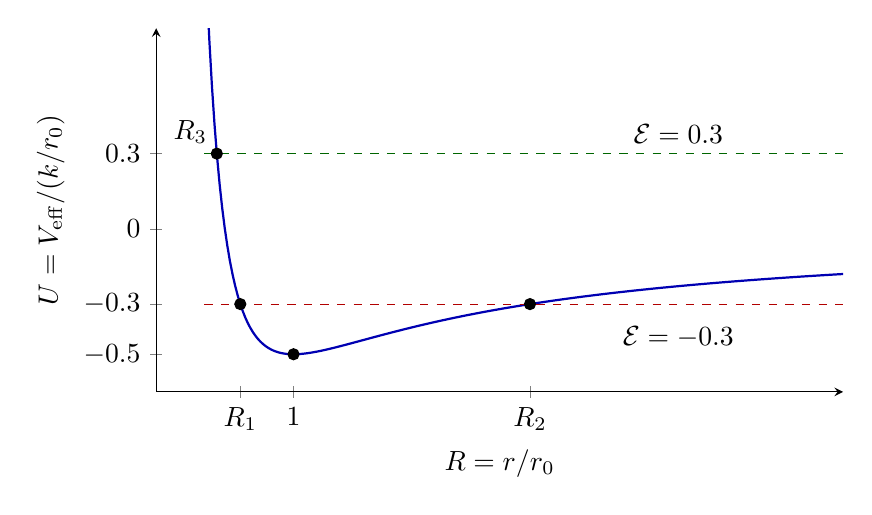
\begin{tikzpicture}
\begin{axis}[width=.85\textwidth,height=6.2cm,axis lines=left,
 xlabel={$R=r/r_0$},ylabel={$U=V_{\rm eff}/(k/r_0)$},xmin=0,xmax=5,ymin=-.65,ymax=.8,
 xtick={.6126,1,2.7208},xticklabels={$R_1$,$1$,$R_2$},ytick={-.5,-.3,0,.3}]
\addplot[thick,blue!70!black,domain=.35:5,samples=250] {-1/x+.5/x^2};
\addplot[dashed,red!70!black,domain=.35:5] {-.3};
\addplot[dashed,green!40!black,domain=.35:5] {.3};
\addplot[only marks,mark=*] coordinates {(1,-.5) (.612574,-.3) (2.720759,-.3) (.441518,.3)};
\node at (axis cs:3.8,-.43) {$\mathcal E=-0.3$};
\node[above left] at (axis cs:.441518,.3) {$R_3$};\node at (axis cs:3.8,.38) {$\mathcal E=0.3$};
\end{axis}
\end{tikzpicture}
\caption{平方反比吸引势的无量纲有效势 $U=-1/R+1/(2R^2)$，$r_0=J^2/(mk)$。负能量的两个交点给出径向振动范围，正能量只有一个近心转折点；$R=1$ 为圆轨道。标记均由所绘曲线与水平能量线的交点计算。}
\label{fig:effective-potential}
\end{figure}

为了求轨道，下面引入比内方程。令 $u=1/r$。利用
\begin{equation}
\dot r=\dv{r}{\theta}\dot\theta
=-\frac{1}{u^2}\dv{u}{\theta}\,hu^2
=-h\dv{u}{\theta},
\end{equation}
\begin{equation}
\ddot r=\dv{\dot r}{\theta}\dot\theta
=-h\dvv[2]{u}{\theta}\,hu^2
=-h^2u^2\dvv[2]{u}{\theta}.
\end{equation}
代入径向方程 \eqref{eq:radial-eom2}，得
\begin{equation}
-mh^2u^2\left(\dvv[2]{u}{\theta}+u\right)=F(1/u).
\end{equation}
于是
\begin{equation}
\boxed{\;\dvv[2]{u}{\theta}+u
=-\frac{F(1/u)}{mh^2u^2}
=-\frac{mF(1/u)}{J^2u^2}\;}
\label{eq:binet}
\end{equation}
这就是\textbf{比内方程}。它把“求轨道”的问题转化为关于 $u(\theta)$ 的二阶常微分方程。

\begin{mathbox}
比内方程的推导只用了角动量守恒和极坐标运动方程，不依赖于 $F(r)$ 的具体形式。因此在 $J\ne0$、可用单调角度参数的轨道段上，它适用于任意中心力；$J=0$ 的纯径向运动应直接用径向时间方程。若已知 $F(r)$，解出 $u(\theta)$ 即得轨道；反之，若已知轨道 $u(\theta)$，也可反推出中心力 $F(r)$。
\end{mathbox}

\subsection{平方反比引力与开普勒定律}

越靠近太阳，引力越强，行星一般也走得更快。把平方反比力代入轨道方程，可以看到椭圆、等面积和周期关系怎样来自同一模型。

考虑引力
\begin{equation}
F(r)=-\frac{k}{r^2}=-ku^2,\qquad k=GMm.
\end{equation}
代入比内方程：
\begin{equation}
\dvv[2]{u}{\theta}+u=\frac{km}{J^2}\equiv\text{常量}.
\end{equation}
其通解为
\begin{equation}
u=A\cos(\theta-\theta_0)+\frac{km}{J^2}.
\end{equation}
于是
\begin{equation}
r=\frac{p}{1+e\cos(\theta-\theta_0)},\qquad
p=\frac{J^2}{km},\qquad
e=\frac{AJ^2}{km}.
\label{eq:conic}
\end{equation}
以下取 $J\ne0$、$e\ge0$，这是以力心为焦点的圆锥曲线：
\begin{itemize}[leftmargin=2.2em]
  \item $e=0$：圆；
  \item $0<e<1$：椭圆；
  \item $e=1$：抛物线；
  \item $e>1$：双曲线。
\end{itemize}
在近心点 $\theta=\theta_0$，$\dot r=0$、$r_p=p/(1+e)$，故
\[
E=\frac{J^2}{2mr_p^2}-\frac{k}{r_p}
=\frac{k}{2p}\bigl[(1+e)^2-2(1+e)\bigr].
\]
用 $p=J^2/(km)$ 消去 $p$，得到总能量与偏心率的关系
\begin{equation}
E=\frac{mk^2}{2J^2}\left(e^2-1\right).
\label{eq:energy-eccentricity}
\end{equation}
因此 $E<0$ 对应椭圆（束缚态），$E=0$ 对应抛物线（临界逃逸），$E>0$ 对应双曲线（散射态）。

\begin{figure}[htbp]
\centering
\begin{tikzpicture}\begin{axis}[width=.31\textwidth,height=4.6cm,axis equal image,axis lines=middle,xmin=-3.8,xmax=1.6,ymin=-3,ymax=3,ticks=none,title={椭圆},xlabel={$x/p$},ylabel={$y/p$}]
\addplot[thick,blue!70!black,domain=-180:180,samples=200] ({cos(x)/(1+0.6*cos(x))},{sin(x)/(1+0.6*cos(x))});
\fill[orange!80!black] (axis cs:0,0) circle (2pt) node[below left]{$F$};\end{axis}\end{tikzpicture}
\begin{tikzpicture}\begin{axis}[width=.31\textwidth,height=4.6cm,axis equal image,axis lines=middle,xmin=-3.8,xmax=1.6,ymin=-3,ymax=3,ticks=none,title={抛物线},xlabel={$x/p$},ylabel={$y/p$}]
\addplot[thick,blue!70!black,domain=-130:130,samples=200] ({cos(x)/(1+1*cos(x))},{sin(x)/(1+1*cos(x))});
\fill[orange!80!black] (axis cs:0,0) circle (2pt) node[below left]{$F$};\end{axis}\end{tikzpicture}
\begin{tikzpicture}\begin{axis}[width=.31\textwidth,height=4.6cm,axis equal image,axis lines=middle,xmin=-3.8,xmax=1.6,ymin=-3,ymax=3,ticks=none,title={双曲线},xlabel={$x/p$},ylabel={$y/p$}]
\addplot[thick,blue!70!black,domain=-115:115,samples=200] ({cos(x)/(1+1.5*cos(x))},{sin(x)/(1+1.5*cos(x))});
\fill[orange!80!black] (axis cs:0,0) circle (2pt) node[below left]{$F$};\end{axis}\end{tikzpicture}

\caption{统一取焦点为原点、半通径为尺度，分别绘制 $e=0.6,1,1.5$ 的轨道。双曲线只画与该吸引力焦点对应的物理支，不能把另一支也当成同一次引力散射轨迹。}
\label{fig:conics}
\end{figure}

对椭圆，$p=a(1-e^2)$、短半轴 $b=a\sqrt{1-e^2}$，因此 $E=-k/(2a)$。面积速度为 $h/2$，一周面积为 $\pi ab$，于是
\[
T=\frac{2\pi ab}{h},\qquad
h^2=\frac{k}{m}p=GM a(1-e^2),\qquad
T^2=\frac{4\pi^2a^3}{GM}.
\]
这个推导先把力心视为固定。对真实两体相对运动，应把动力学质量换成约化质量、$k=Gm_1m_2$，从而 $k/\mu=G(m_1+m_2)$。此时 $a$ 是两体相对距离轨道的半长轴，而非任意一颗天体关于质心轨道的半长轴。

开普勒三定律可由上述结果导出：
\begin{enumerate}[label=(\arabic*),leftmargin=2.2em]
  \item 行星沿椭圆轨道运动，太阳位于椭圆的一个焦点上；
  \item 行星与太阳的连线在相等时间内扫过相等面积（面积速度守恒）；
  \item 行星公转周期 $T$ 的平方与椭圆半长轴 $a$ 的立方成正比：
  \begin{equation}
  T^2=\frac{4\pi^2a^3}{G(M+m)}.
  \label{eq:kepler3}
  \end{equation}
  当 $M\gg m$ 时，$T^2\approx4\pi^2a^3/(GM)$。
\end{enumerate}

\begin{figure}[htbp]
\centering
\begin{tikzpicture}[>=Stealth,scale=1.35]
\coordinate (F) at (1.2,0);
\draw[thick,blue!70!black] (0,0) ellipse (2 and 1.6);
\fill[blue!12] (F)--(2,0) plot[domain=0:65.712221235,samples=60] ({2*cos(\x)},{1.6*sin(\x)})--cycle;
\fill[red!12] (F)--(-2,0) plot[domain=180:201.678498205,samples=60] ({2*cos(\x)},{1.6*sin(\x)})--cycle;
\draw[thick] (F)--(2,0);\draw[thick] (F)--({2*cos(65.712221235)},{1.6*sin(65.712221235)});
\draw[thick] (F)--(-2,0);\draw[thick] (F)--({2*cos(201.678498205)},{1.6*sin(201.678498205)});
\fill[orange!80!black] (F) circle (2pt) node[below right]{$F$};
\node at (1.4,.4) {$A_1$};\node at (-1,-.25) {$A_2$};
\end{tikzpicture}
\caption{两块区域由椭圆弧和焦点连线围成。取 $a=2,b=1.6,e=0.6$，偏近点角区间按相等的 $\Delta(E-e\sin E)$ 计算，从而表示相等时间与相等扫掠面积，不能以任意直线三角形替代扇形。}
\label{fig:kepler-area}
\end{figure}

\subsection{有效势能、轨道分类与稳定性}

把同一角动量下的转动动能和原来的势能合在一起，半径便像一个一维坐标那样运动。有效势的最低点给出可能的稳定圆轨道。

由式 \eqref{eq:central-energy}，径向运动等价于一维问题：
\begin{equation}
\frac12m\dot r^2+V_{\rm eff}(r)=E.
\end{equation}
圆轨道满足
\begin{equation}
V_{\rm eff}'(r_0)=0
\quad\Longleftrightarrow\quad
F(r_0)=-\frac{J^2}{mr_0^3}.
\label{eq:circular-condition}
\end{equation}
这就是“中心力提供向心力”的条件。圆轨道的能量为
\begin{equation}
E_0=V_{\rm eff}(r_0).
\end{equation}
令 $r=r_0+\delta r$，在固定角动量下展开 $m\ddot r=-V_{\rm eff}'(r)$：
\[
m\ddot{\delta r}=-V_{\rm eff}''(r_0)\delta r+O(\delta r^2).
\]
所以线性径向振动频率为 $\omega_r^2=V_{\rm eff}''(r_0)/m$，稳定性要求
\begin{equation}
V_{\rm eff}''(r_0)>0.
\label{eq:stability}
\end{equation}
对于平方反比引力，
\begin{equation}
r_0=\frac{J^2}{mk},\qquad
E_0=-\frac{mk^2}{2J^2},\qquad
\omega_0=\frac{J}{mr_0^2}=\sqrt{\frac{k}{mr_0^3}}.
\end{equation}

\begin{example}[月球探测器的霍曼转移]
月球探测器在半径 $r_1$ 的环月圆轨道上运行，欲通过霍曼转移进入半径 $r_2>r_1$ 的共面圆轨道。求两次点火所需的速度增量，并估算从 $100\,\mathrm{km}$ 到 $1000\,\mathrm{km}$ 环月圆轨道所需的总 $\Delta v$。

\begin{center}
\begin{tikzpicture}[>=Stealth,scale=0.95]
  \fill[gray!25] (0,0) circle (0.55);
  \node at (0,-0.85) {月球};
  \draw[blue!55,thick] (0,0) circle (1.2);
  \draw[blue!35,thick] (0,0) circle (2.0);
  \draw[red!75!black,thick] (-0.4,0) ellipse (1.6 and 1.549193);
  \fill (1.2,0) circle (2pt);
  \fill (-2.0,0) circle (2pt);
  \draw[->,thick,green!45!black] (1.2,0)--++(0,0.55) node[right]{$\Delta v_1$};
  \draw[->,thick,green!45!black] (-2.0,0)--++(0,-0.45) node[left]{$\Delta v_2$};
  \node[blue!55] at (0.9,1.10) {$r_1$};
  \node[blue!35] at (1.45,1.80) {$r_2$};
\end{tikzpicture}
\end{center}

解：霍曼转移轨道是一个椭圆，近月点为 $r_1$、远月点为 $r_2$，半长轴为
\[
a=\frac{r_1+r_2}{2}.
\]
由椭圆能量 $E=-m\mu_M/(2a)$ 与任意点能量 $E=mv^2/2-m\mu_M/r$ 相等，消去 $E$ 得活力公式
\[
v^2=\mu\left(\frac{2}{r}-\frac{1}{a}\right),
\]
其中本例 $\mu=GM$ 为月球引力参数，与前文约化质量符号同形，但物理量、单位不同；以下数值用 $\mu_M$ 表示。第一次点火在 $r_1$ 处，把圆轨道速度
\[
v_1^c=\sqrt{\frac{\mu}{r_1}}
\]
加速到转移轨道近月点速度
\[
v_1^t=\sqrt{\mu\left(\frac{2}{r_1}-\frac{1}{a}\right)},
\]
故
\[
\Delta v_1=v_1^t-v_1^c .
\]
到达远月点 $r_2$ 后，转移轨道速度为
\[
v_2^t=\sqrt{\mu\left(\frac{2}{r_2}-\frac{1}{a}\right)},
\]
而目标圆轨道速度为
\[
v_2^c=\sqrt{\frac{\mu}{r_2}}.
\]
第二次点火使探测器加速到 $v_2^c$，于是
\[
\Delta v_2=v_2^c-v_2^t .
\]
总速度增量为 $\Delta v=\Delta v_1+\Delta v_2$。

转移飞行时间为椭圆半周期 $t_{\rm tr}=\pi\sqrt{a^3/\mu_M}$。本例计算约为 $4.91\times10^3\,\mathrm{s}$。

取月球半径 $R_M=1737.4\,\mathrm{km}$、$\mu_M=4.902800118\times10^{12}\,\mathrm{m^3/s^2}$。对 $r_1=R_M+100\,\mathrm{km}$、$r_2=R_M+1000\,\mathrm{km}$，计算得
\[
\Delta v_1\approx153\,\mathrm{m/s},\qquad
\Delta v_2\approx139\,\mathrm{m/s},
\]
故总 $\Delta v\approx0.29\,\mathrm{km/s}$。霍曼转移的两次点火都沿速度方向，在球对称两体模型、瞬时切向双脉冲、指定两圆轨道之间具有标准的低速度增量性质；不能推广为允许任意脉冲数及中间轨道时的全局最优。实际任务需另计摄动、有限推力和误差。采用的月球参数来源于 JPL，见章末来源；轨道高度是教学设定，不对应特定任务。
\end{example}

有效势能还决定圆轨道的稳定性。考虑一般幂次中心力
\begin{equation}
F(r)=-\frac{k}{r^n}=-ku^n .
\end{equation}
由比内方程，圆轨道满足
\begin{equation}
ku_0^{n-3}=mh^2 .
\end{equation}
令 $u=u_0+\xi$，线性化得
\begin{equation}
\dvv[2]{\xi}{\theta}+(3-n)\xi=0 .
\label{eq:stability-perturb}
\end{equation}
因此圆轨道稳定的条件是
\begin{equation}
\boxed{\;n<3\;}
\label{eq:stability-condition}
\end{equation}
当 $n<3$ 时，径向扰动表现为简谐振荡，轨道在圆附近振荡；当 $n>3$ 时出现指数增长；$n=3$ 时线性方程为 $\xi''=0$，是退化临界情况，扰动可线性增长，不能称为指数增长或据此断言稳定。平方反比引力 $n=2$ 是稳定情形，且扰动频率与角频率相同，轨道闭合（伯特兰定理的一个特例）。


\begin{example}[幂次势的圆轨道与径向频率]
质量为 $m$ 的质点在势能 $V(r)=\beta r^k$ 中运动，角动量为 $L$。求圆轨道半径与径向微振动频率，并验证拱点角公式。

解：有效势能为
\[
V_{\rm eff}(r)=\frac{L^2}{2mr^2}+\beta r^k .
\]
设 $L\ne0$、$\beta k>0$ 且 $k\ne-2$，圆轨道满足 $V_{\rm eff}'(r_0)=0$：
\[
-\frac{L^2}{mr_0^3}+\beta k r_0^{k-1}=0
\quad\Longrightarrow\quad
r_0=\left(\frac{L^2}{m\beta k}\right)^{1/(k+2)} .
\]
在 $r_0$ 附近作小振动，径向频率为
\[
\omega_r^2=\frac{V_{\rm eff}''(r_0)}{m}
=\frac{1}{m}\left[\frac{3L^2}{mr_0^4}+\beta k(k-1)r_0^{k-2}\right].
\]
利用圆轨道条件 $L^2/(mr_0^3)=\beta k r_0^{k-1}$，得
\[
\omega_r^2=\frac{\beta k(k+2)}{m}r_0^{k-2}
=(k+2)\omega_0^2,
\]
其中 $\omega_0=L/(mr_0^2)$ 是圆轨道的角频率。稳定性还要求 $k>-2$。在小扰动极限，从近心点到远心点的拱点角为
\[
\Psi=\pi\frac{\omega_0}{\omega_r}
=\frac{\pi}{\sqrt{k+2}} .
\]
当 $k=2$ 时 $\Psi=\pi/2$，当 $k=-1$ 时 $\Psi=\pi$；其他幂次也可能给出有理频率比，但近圆有理比只约束线性近似，不能保证有限振幅的所有轨道闭合。这个结果正是伯特兰定理证明的起点。
\end{example}

\subsection{进一步探索：伯特兰定理与轨道进动}
近圆轨道每次到达最近点时，方向未必一样。比较半径往复的周期与绕中心转动的周期，便可判断近心方向是否逐圈移动。

圆轨道稳定不等于所有轨道闭合。本小节超出首次学习所必需的核心内容，使用比内方程与小振幅展开，说明闭合要求有多严格；所需基础是泰勒展开和三角恒等式。
\begin{theorem}[伯特兰定理的通常正则情形]
对光滑吸引中心势，在可形成稳定圆轨道的连通半径范围内，若所有非碰撞束缚轨道都闭合，则允许的势只有 $V=-k/r$ 与 $V=kr^2/2$（$k>0$），相差常数不影响运动。这里要求一族稳定圆轨道与其邻近束缚轨道，不能用仅存在孤立闭轨道替代。
\end{theorem}

\paragraph{必要条件：近圆频率比必须保持不变。}
由前节径向小振动，近圆轨道的半径向周期转角为
\begin{equation}\label{eq:apsidal-angle}
\Psi_0=\pi\left[3+\frac{r_0V''(r_0)}{V'(r_0)}\right]^{-1/2}.
\end{equation}
闭合要求径向与角向周期可公度。若对连续变化的轨道参数始终闭合，连续变化的频率比又只能取有理数，故它必须是常数。令中括号为 $C>0$，则
\[
rV''=(C-3)V',\qquad V'=A r^{C-3}.
\]
在该连通范围内，势能为幂次 $V=\beta r^k+\mathrm{const}$，$k=C-2>-2$；$k=0$ 的极限形式为对数势 $A\ln r$。仅检验近圆运动还不能排除其他有理频率比。

\paragraph{再进一步：振幅变化不能改变频率比。}
对幂次势，令 $u=u_0(1+x)$，用圆轨道条件消去系数，比内方程变成
\[
x''+1+x=(1+x)^{-k-1},
\]
撇号表示对方位角 $\theta$ 求导。展开到三阶：
\[
x''+w_0^2x=a_2x^2+a_3x^3+O(x^4),\quad
w_0^2=k+2,
\]
\[
a_2=\frac{(k+1)(k+2)}2,\qquad
a_3=-\frac{(k+1)(k+2)(k+3)}6.
\]
设 $\zeta=w\theta$，用小振幅参数 $\epsilon$ 写为
\[
x=\epsilon\cos\zeta+\epsilon^2(c_0+c_2\cos2\zeta)+O(\epsilon^3),\quad
w=w_0(1+d\epsilon^2+\cdots).
\]
二阶常数项及倍频项给出 $c_0=a_2/(2w_0^2)$、$c_2=-a_2/(6w_0^2)$。三阶 $\cos\zeta$ 项若不消去，会产生非周期的世俗项；其系数条件为
\[
-2w_0^2d=2a_2(c_0+c_2/2)+3a_3/4,
\]
于是
\[
d=-\frac{5a_2^2}{12w_0^4}-\frac{3a_3}{8w_0^2}
=\frac{(k+1)(2-k)}{24}.
\]
若所有小而有限振幅轨道均闭合，频率比不能随连续振幅改变，必须有 $d=0$。故只剩 $k=-1$ 或 $k=2$；对数势对应的比内展开取 $k=0$，其 $d\ne0$，亦被排除。这给出了所述正则情形中的筛选条件。

\paragraph{充分性：两个候选确实闭合。}
平方反比吸引势的非碰撞束缚轨道已证明为焦点椭圆。对各向同性谐振子，$\ddot x+\omega^2x=\ddot y+\omega^2y=0$，通过旋转平面坐标并选择时间原点，可写成 $x=A\cos\omega t,y=B\sin\omega t$，轨道是以力心为中心的椭圆；径向退化轨道为线段。因此两个候选均满足闭合要求。

\begin{physicsbox}
开普勒椭圆的长轴方向固定，比单纯的角动量守恒更强。在 $V=-k/r$ 中，还存在沿近心方向的守恒量 $\bA=\bp\times\bJ-mk\er$。其守恒可在章末习题直接检验。隐藏守恒量说明为何这两类势具有特别简单的轨道；更一般的中心势通常允许拱点进动。
\end{physicsbox}
\begin{modernbox}[title={近圆拱点进动的适用范围}]
对幂次势，$\Psi_0=\pi/\sqrt{k+2}$ 只是在近圆极限的半径向周期转角。从一个近心点到下一个近心点的方位增量约为 $2\Psi_0$。对接近开普勒势的运动，常用进动约定为 $\Delta\varpi\simeq2\Psi_0-2\pi$。这不是一般偏心轨道的精确公式，也不能直接用来计算广义相对论进动。

有限振幅的精确拱点角应从能量积分计算：
\begin{equation}\label{eq:apsidal-integral}
\Psi(E,J)=\int_{r_-}^{r_+}
\frac{|J|\,\dd r}{r^2\sqrt{2m[E-V(r)]-J^2/r^2}}.
\end{equation}
这里从近心到远心只积分一次；再乘2才是一个完整径向周期的转角。进一步阅读可用本章参考的中心力讲义，第\ref{sec:kepler-action}节再用径向作用变量讨论周期。
\end{modernbox}

\subsection{散射截面与卢瑟福散射}

把一束粒子打向靶，瞄得越偏，经过靶附近时通常偏转得越少。用入射位置的面积去对应出射角的范围，就得到散射截面的含义。

考虑质量为 $m$ 的粒子以初速 $v_0$、瞄准距 $b$ 射向力心。角动量和能量为
\begin{equation}
J=mv_0b,\qquad E=\frac12mv_0^2 .
\end{equation}
粒子在中心力场中偏转，出射方向与入射方向的夹角 $\Theta$ 称为\textbf{散射角}。所有瞄准距在 $b\sim b+\dd b$ 内的粒子，被散射到 $\Theta\sim\Theta+\dd\Theta$ 的立体角内。在轴对称、每个散射角只对应一个瞄准距的分支上，入射环带面积为 $\dd\sigma=2\pi b|\dd b|$，出射角环的立体角为 $\dd\Omega=2\pi\sin\Theta|\dd\Theta|$。两者相除，定义\textbf{微分散射截面}
\begin{equation}
\dv{\sigma}{\Omega}=\frac{b}{\sin\Theta}\left|\dv{b}{\Theta}\right|,
\label{eq:cross-section}
\end{equation}
若多个不同瞄准距产生同一散射角，微分截面应把各分支贡献相加。总截面为
\begin{equation}
\sigma=\int \dv{\sigma}{\Omega}\,\dd\Omega
=2\pi\int_0^\pi \frac{b}{\sin\Theta}\left|\dv{b}{\Theta}\right|\sin\Theta\,\dd\Theta .
\end{equation}

\begin{figure}[htbp]
\centering
\begin{tikzpicture}[>=Stealth,scale=1.05]
\coordinate (C) at (0.666667,0);
\draw[dashed,gray] (C)--++(-60:3.5);
\draw[dashed,gray] (C)--++(60:3.5);
\draw[dashed,gray] (C)--++(120:1.6);
\draw[very thick,blue!65!black,domain=-48:48,samples=160]
 plot ({cos(\x)/(2*cos(\x)-1)},{sin(\x)/(2*cos(\x)-1)});
\fill[orange!80!black] (0,0) circle (2.5pt) node[left]{力心};
\draw[->,thick,red!70!black] (2.07,-2.43)--(1.62,-1.65) node[right]{入射};
\draw[->,thick,red!70!black] (1.62,1.65)--(2.07,2.43) node[right]{出射};
\draw[->,thick] (C)++(60:.9) arc (60:120:.9);
\node at (.67,1.2) {$\Theta$};
\draw[<->] (0,0)--(.5,-.288675) node[midway,below left]{$b$};
\end{tikzpicture}
\caption{解析排斥轨道 $r=p/(e\cos\theta-1)$ 的实例，取 $p=1,e=2$。虚线为真正的渐近线；散射角比较入射、出射的速度方向，本例为 $60^\circ$。$b$ 是力心到入射渐近线的垂距。}
\label{fig:scattering}
\end{figure}

对于库仑排斥力
\begin{equation}
F(r)=\frac{k}{r^2},\qquad k=\frac{q_1q_2}{4\pi\varepsilon_0},
\end{equation}
以下假设固定重靶、点电荷、非相对论且无屏蔽，取 $k>0$。以近心点方向为极轴，比内方程的排斥解可写为
\[
r=\frac{p}{e\cos\theta-1},\qquad
p=\frac{J^2}{mk},\quad
e^2=1+\frac{2EJ^2}{mk^2}.
\]
无穷远的渐近角满足 $\cos\theta_\infty=1/e$。入射速度指向近心区、出射速度离开，因此速度偏转角为 $\Theta=\pi-2\theta_\infty$，不是直接把两条无向直线的小夹角当作偏转角。于是
\[
\cot(\Theta/2)=\tan\theta_\infty=\sqrt{e^2-1}
=\frac{mv_0^2b}{k},
\]
散射角与瞄准距满足
\begin{equation}
b=\frac{k}{mv_0^2}\cot\frac{\Theta}{2}
=\frac{k}{2E}\cot\frac{\Theta}{2}.
\label{eq:rutherford-b}
\end{equation}
对 $b=(k/2E)\cot(\Theta/2)$ 求导，
\[
\left|\frac{\dd b}{\dd\Theta}\right|=\frac{k}{4E}\csc^2(\Theta/2).
\]
代入式 \eqref{eq:cross-section}，用 $\sin\Theta=2\sin(\Theta/2)\cos(\Theta/2)$ 化简，得\textbf{卢瑟福散射公式}
\begin{equation}
\boxed{\;
\dv{\sigma}{\Omega}
=\left(\frac{k}{4E}\right)^2
\frac{1}{\sin^4(\Theta/2)}
=\left(\frac{q_1q_2}{16\pi\varepsilon_0E}\right)^2
\frac{1}{\sin^4(\Theta/2)}
\;}
\label{eq:rutherford}
\end{equation}
总截面发散，反映库仑力是长程力；实验报告通常给定非零的最小散射角，屏蔽也可改变小角行为。对 $\Theta\ge\Theta_{\min}>0$，积分截面为 $\sigma=\pi[k/(2E)]^2\cot^2(\Theta_{\min}/2)$，与 $\pi b_{\max}^2$ 一致。不能只凭“探测器有限大小”就消除包含零角的长程发散。

\begin{example}[月球探测器与微陨石的刚球散射]
把月球探测器与微陨石的碰撞简化为半径为 $a$ 的刚性球：由 $b=a\sin\varphi$、$\Theta=\pi-2\varphi$ 得
\[
b=a\cos\frac{\Theta}{2},\qquad
\dv{\sigma}{\Omega}
=\frac{b}{\sin\Theta}\left|\dv{b}{\Theta}\right|
=\frac{a^2}{4}.
\]
总截面 $\sigma=\pi a^2$，恰为几何截面积，可用于估算微陨石撞击探测器的概率。

在轴对称入射束中，入射环带截面是 $2\pi b|\dd b|$，对应的散射立体角是 $2\pi\sin\Theta\,\dd\Theta$。所需导数为
\[
\left|\frac{\dd b}{\dd\Theta}\right|=\frac a2\sin\frac\Theta2 .
\]
用 $\sin\Theta=2\sin(\Theta/2)\cos(\Theta/2)$ 约去半角因子，比值即为 $a^2/4$。将常数对 $4\pi$ 立体角积分即可复核总截面。
\end{example}

\begin{modernbox}
卢瑟福散射是经典力学最著名的“判决性实验”之一。大角度散射对短距离相互作用敏感，因而可以用来检验原子内部电荷分布模型。今天，散射截面仍是粒子物理、核物理和冷原子物理中探测相互作用的基本工具；量子力学中的卢瑟福公式在库仑势下与经典结果形式上一致。
\end{modernbox}

\subsection{潮汐力}

月球对地球不同位置的引力略有差别。先减去地心也受到的那一份，再比较近端和远端，就能分清潮汐作用与整体加速。

潮汐力不是一种新的基本力，而是引力场在有限大小物体上的\emph{差分}效应。设外引力场为 $\bg(\br)$，物体上相距 $\Delta\br$ 的两点加速度之差为
\begin{equation}
\Delta\ba=\bg(\br+\Delta\br)-\bg(\br)
\approx(\Delta\br\cdot\nabla)\bg .
\label{eq:tidal-def}
\end{equation}
对于点质量 $M$ 的引力场 $\bg=-GM\br/r^3$，先求雅可比 $\partial g_i/\partial x_j=GM(3x_ix_j/r^5-\delta_{ij}/r^3)$，再乘以 $\Delta x_j$，得到
\begin{equation}
\Delta\ba=\frac{GM}{r^3}\left[3(\Delta\br\cdot\hat{\br})\hat{\br}-\Delta\br\right].
\label{eq:tidal-acceleration}
\end{equation}
沿径向（$\Delta\br\parallel\hat{\br}$）有
\[
\Delta a_r=+\frac{2GM}{r^3}\Delta r,
\]
物体被\emph{拉伸}；沿垂直方向（$\Delta\br\perp\hat{\br}$）有
\[
\Delta a_\perp=-\frac{GM}{r^3}\Delta r_\perp,
\]
物体被\emph{压缩}。这正是潮汐隆起的几何来源：地球面向月球和背向月球的两侧都被“拉出去”，给出理想平衡潮汐的拉伸方向；真实海潮还受海盆、海岸及耗散动力学影响。

\begin{figure}[htbp]
\centering
\begin{tikzpicture}[>=Stealth,scale=1.0]
  \draw[blue!20,thick] (0,0) circle (1.5);
  \draw[dashed] (-2.4,0)--(4.2,0);
  \draw[gray!60,thick] (5.4,0) circle (0.55);
  \node at (5.4,-1.0) {月球};
  \node at (0,-1.9) {地球};
  \fill (1.5,0) circle (2pt);
  \fill (-1.5,0) circle (2pt);
  \fill (0,1.5) circle (2pt);
  \fill (0,-1.5) circle (2pt);
  \draw[->,very thick,red!75!black] (1.5,0)--++(0.85,0);
  \draw[->,very thick,red!75!black] (-1.5,0)--++(-0.85,0);
  \draw[->,very thick,blue!70!black] (0,1.5)--++(0,-0.8);
  \draw[->,very thick,blue!70!black] (0,-1.5)--++(0,0.8);
  \node[red!75!black] at (2.45,0.35) {拉伸};
  \node[blue!70!black] at (0.55,0.95) {压缩};
\end{tikzpicture}
\caption{潮汐力的几何图像。沿地月连线方向，引力差把地球两侧向外拉（拉伸）；垂直方向则向内压（压缩），形成两个潮汐隆起。}
\label{fig:tidal}
\end{figure}

潮汐力的大小随距离迅速衰减：
\begin{equation}
|\Delta\ba|\sim\frac{GM}{r^3}\,\Delta r .
\end{equation}
因此潮汐效应在近距离天体系统中特别显著。

\begin{itemize}[leftmargin=2.2em]
  \item \textbf{潮汐锁定}：潮汐隆起受到引力转矩，使天体自转角速度逐渐趋向公转角速度。月球已被地球潮汐锁定，以近乎同一面朝向地球，观测中的天平动仍会改变可见区域；潮汐耗散也会交换自转与轨道角动量。
  \item \textbf{洛希极限}：当小物体的自身引力不足以抵抗主星的潮汐拉伸时，它会被撕裂。设小物体半径为 $R$、密度为 $\rho$，主星质量为 $M$，则潮汐撕裂的临界距离约为
  \begin{equation}
  d_{\rm Roche}\sim R\left(\frac{2M}{m}\right)^{1/3}
  =\left(\frac{3M}{2\pi\rho}\right)^{1/3}
  \propto \rho^{-1/3}.
  \end{equation}
  对理想同步流体卫星，常用模型写成 $d_{\rm Roche}\simeq2.44R_M(\rho_M/\rho)^{1/3}$，其中 $R_M,\rho_M$ 为主星半径、平均密度。这个系数对应另一套流体平衡模型，不能直接乘到上述点对点拉伸估算式上。土星环、彗星碎裂等现象都与洛希极限有关。
  \item \textbf{潮汐加热}：若轨道偏心率较大，潮汐形变随时间变化，机械能转化为内能。木卫二冰壳下的海洋、木卫一的火山活动，都与潮汐加热密切相关。
\end{itemize}

\begin{modernbox}
在广义相对论中，潮汐力对应时空曲率引起的\emph{测地线偏离}。等效原理只能在一个自由落体参考系的局部邻域内消去引力加速度，但无法消去潮汐力；因此潮汐力是“引力的不可消除部分”，也是探测引力波的基本原理：引力波通过时，空间中的自由检验质量会发生差分振荡。
\end{modernbox}


\subsection{拉格朗日点与限制性三体问题}

如果在随两个主天体一起转的坐标系中看，有些位置上的小物体可以相对两者保持不动。找出这些平衡点后，还要另问轻轻推离会发生什么。

拉格朗日点是限制性三体问题中最著名的结果。设两个大质量天体 $M_1,M_2$ 绕共同质心作圆轨道，间距为 $a$，角速度为 $\Omega$，满足
\begin{equation}
\Omega^2=\frac{G(M_1+M_2)}{a^3}.
\end{equation}
第三个物体质量 $m\ll M_1,M_2$，它对两个大天体的引力影响可以忽略，但仍在它们的引力场中运动。这就是\textbf{限制性三体问题}。

取随两个大天体一起转动的参考系，令 $M_1$ 位于 $x=0$，$M_2$ 位于 $x=a$。总质量 $M=M_1+M_2$，质心位于 $x=a\mu$，其中
\begin{equation}
\mu=\frac{M_2}{M_1+M_2}.
\end{equation}
第三体的坐标为 $(x,y)$，到两个大天体的距离分别为
\begin{equation}
r_1=\sqrt{x^2+y^2},\qquad
r_2=\sqrt{(x-a)^2+y^2}.
\end{equation}
在转动系中，第三体受到两个引力、离心力和科里奥利力。科里奥利力不做功，不贡献势能；单位质量的\textbf{有效势能}为
\begin{equation}
\Phi(x,y)=-\frac{GM_1}{r_1}-\frac{GM_2}{r_2}
-\frac12\Omega^2\left[(x-a\mu)^2+y^2\right].
\label{eq:lagrange-effective}
\end{equation}
第三体的运动方程为
\begin{equation}
\ddot x-2\Omega\dot y=-\pdv{\Phi}{x},\qquad
\ddot y+2\Omega\dot x=-\pdv{\Phi}{y}.
\label{eq:lagrange-eom}
\end{equation}
平衡点满足 $\dot x=\dot y=0$、$\ddot x=\ddot y=0$，因此
\begin{equation}
\pdv{\Phi}{x}=0,\qquad
\pdv{\Phi}{y}=0.
\label{eq:lagrange-equilibrium}
\end{equation}
这些平衡点就是\textbf{拉格朗日点}。

\paragraph{共线拉格朗日点 $L_1,L_2,L_3$.}
先令 $y=0$。在 $M_1,M_2$ 之间的 $L_1$ 点，$0<x<a$，有
\[
\pdv{\Phi}{x}
=\frac{GM_1}{x^2}-\frac{GM_2}{(a-x)^2}
-\Omega^2(x-a\mu)=0.
\]
令 $x=au$，并利用 $\Omega^2=GM/a^3$，得到无量纲方程
\begin{equation}
\frac{1-\mu}{u^2}-\frac{\mu}{(1-u)^2}-(u-\mu)=0,
\qquad 0<u<1.
\label{eq:L1-equation}
\end{equation}
这是关于 $u$ 的代数方程，一般没有简单的闭式解，但可用数值方法求解。对小的质量比 $\mu$，近似有
\begin{equation}
u_{L1}\approx1-\left(\frac{\mu}{3}\right)^{1/3},\qquad
u_{L2}\approx1+\left(\frac{\mu}{3}\right)^{1/3},\qquad
u_{L3}\approx-1+\frac{7}{12}\mu .
\end{equation}
因此 $L_1$ 位于两天体之间、靠近较小天体；$L_2$ 位于较小天体外侧；$L_3$ 位于较大天体另一侧。三个共线点都在两体连线上。

\paragraph{三角拉格朗日点 $L_4,L_5$.}
令
\begin{equation}
x=\frac a2,\qquad y=\pm\frac{\sqrt3}{2}a .
\end{equation}
此时 $r_1=r_2=a$，即 $L_4,L_5$ 与 $M_1,M_2$ 构成等边三角形。直接代入式 \eqref{eq:lagrange-equilibrium} 验证：
\[
\pdv{\Phi}{x}
=\frac{GM_1(a/2)}{a^3}
+\frac{GM_2(-a/2)}{a^3}
-\Omega^2\left(\frac a2-a\mu\right)
=0,
\]
\[
\pdv{\Phi}{y}
=\frac{GM_1(\sqrt3a/2)}{a^3}
+\frac{GM_2(\sqrt3a/2)}{a^3}
-\Omega^2\frac{\sqrt3a}{2}
=0.
\]
所以 $L_4,L_5$ 确实是平衡点，它们位于两体连线的两侧，与两天体构成等边三角形。

\begin{center}
\begin{tikzpicture}[>=Stealth,scale=.82]
\fill[blue!6] (-2,0)--(0,3.464102)--(2,0)--cycle;
\fill[blue!6] (-2,0)--(0,-3.464102)--(2,0)--cycle;
\draw[dashed] (-6,0)--(4.2,0);
\draw[dashed] (-2,0)--(0,3.464102)--(2,0)--(0,-3.464102)--cycle;
\fill[blue!65!black] (-2,0) circle (4pt) node[below]{$M_1$};
\fill[orange!85!black] (2,0) circle (3pt) node[below]{$M_2$};
\fill[green!40!black] (0,3.464102) circle (2.5pt) node[above]{$L_4$};
\fill[green!40!black] (0,-3.464102) circle (2.5pt) node[below]{$L_5$};
\fill[red!70!black] (0.8361404400928096,0) circle (2pt) node[above]{$L_1$};
\fill[red!70!black] (3.438799331609326,0) circle (2pt) node[above]{$L_2$};
\fill[red!70!black] (-5.76643563428424,0) circle (2pt) node[above]{$L_3$};
\node at (-1,-4) {$\mu=0.1$，共线位置由平衡方程数值求得};
\end{tikzpicture}
\end{center}

\paragraph{稳定性分析.}
平衡点是否存在与是否稳定是两个问题。令 $x=x_0+\xi$、$y=y_0+\eta$，在平衡点附近线性化式 \eqref{eq:lagrange-eom}：
\begin{equation}
\ddot\xi-2\Omega\dot\eta
=-\Phi_{xx}\xi-\Phi_{xy}\eta,
\end{equation}
\begin{equation}
\ddot\eta+2\Omega\dot\xi
=-\Phi_{xy}\xi-\Phi_{yy}\eta,
\end{equation}
其中二阶偏导数在平衡点取值。设指数模态 $\xi,\eta\propto e^{\lambda t}$，代入后得到关于 $\xi,\eta$ 的齐次线性方程组。要有非零解，系数行列式必须为零：
\begin{equation}
\begin{vmatrix}
\lambda^2+\Phi_{xx} & -2\Omega\lambda+\Phi_{xy}\\
2\Omega\lambda+\Phi_{xy} & \lambda^2+\Phi_{yy}
\end{vmatrix}=0 .
\end{equation}
展开行列式，就得到特征方程
\begin{equation}
\lambda^4+\left(\Phi_{xx}+\Phi_{yy}+4\Omega^2\right)\lambda^2
+\Phi_{xx}\Phi_{yy}-\Phi_{xy}^2=0.
\label{eq:lagrange-characteristic}
\end{equation}

对共线点 $L_1,L_2,L_3$，令 $A=GM_1/r_1^3+GM_2/r_2^3$。在 $y=0$ 直接微分可得 $\Phi_{xy}=0$、$\Phi_{xx}=-2A-\Omega^2$、$\Phi_{yy}=A-\Omega^2$。在两主星之间，$r_1,r_2<a$，故 $A>G(M_1+M_2)/a^3=\Omega^2$。对外侧平衡点，记 $x_C=a\mu$，将 $\Phi_x=0$ 写成
\[
(A-\Omega^2)(x-x_C)
=G M_2(a-x_C)(r_2^{-3}-r_1^{-3}).
\]
右边用到了 $M_1x_C=M_2(a-x_C)$。右侧外点有 $r_2<r_1$ 且 $x-x_C>0$，左侧外点两处符号同时反转，因而两处也有 $A>\Omega^2$。于是
\begin{equation}
\Phi_{xx}\Phi_{yy}-\Phi_{xy}^2<0,
\end{equation}
把特征方程视为关于 $u=\lambda^2$ 的二次式。常数项为负，两个根必为异号实数，正的 $u$ 给出增长指数 $\lambda=+\sqrt u$，因此平衡不稳定。这正是为什么航天器不能长期“停”在 $L_1,L_2,L_3$ 上，而需要主动轨道保持。

对三角点，设 $\boldsymbol d_i$ 是从第 $i$ 个主星指向第三体的位移。引力势 $-GM_i/r_i$ 的二阶导矩阵为 $GM_i(I/r_i^3-3\boldsymbol d_i\boldsymbol d_i^{\mathsf T}/r_i^5)$。因 $r_1=r_2=a$，两项的单位矩阵部分恰与离心势的 $-\Omega^2I$ 抵消。将 $\boldsymbol d_1/a=(1/2,\pm\sqrt3/2)$ 和 $\boldsymbol d_2/a=(-1/2,\pm\sqrt3/2)$ 代入余下的外积，得
\begin{equation}
\Phi_{xx}=-\frac34\Omega^2,\qquad
\Phi_{yy}=-\frac94\Omega^2,\qquad
\Phi_{xy}=\mp\frac{3\sqrt3}{4}(1-2\mu)\Omega^2.
\end{equation}
代入式 \eqref{eq:lagrange-characteristic}，得到
\begin{equation}
\lambda^4+\Omega^2\lambda^2
+\frac{27}{4}\mu(1-\mu)\Omega^4=0.
\label{eq:L4-characteristic}
\end{equation}
令 $u=\lambda^2$，则
\begin{equation}
u^2+\Omega^2u+\frac{27}{4}\mu(1-\mu)\Omega^4=0.
\end{equation}
两根之和为 $-\Omega^2<0$，乘积为 $\frac{27}{4}\mu(1-\mu)\Omega^4>0$，若判别式严格为正且 $0<\mu<1$，则两个根为不同的负实数。临界时 $u=-\Omega^2/2$ 为重根。对应 $\lambda=\pm i\Omega/\sqrt2$ 时，前面的二阶模态矩阵行列式为零且非零（非对角元含非零虚部），故每个重根只有一个独立振型。一阶系统因此有含 $t e^{\lambda t}$ 的广义模态，临界扰动并非全都保持有界。判别式为
\begin{equation}
\Omega^4\left[1-27\mu(1-\mu)\right],
\end{equation}
故线性有界稳定的条件为
\begin{equation}
1-27\mu(1-\mu)>0.
\end{equation}
如果没有科里奥利力，$L_4,L_5$ 是有效势能的极大点，运动不稳定；正是科里奥利力在质量比足够小时把运动“拧”成有界振荡。
因此在线性近似中稳定的条件为
\begin{equation}
\mu<\frac12\left(1-\sqrt{\frac{23}{27}}\right)
\approx0.03852
\quad\text{或}\quad
\mu>0.96148 .
\end{equation}
对于 $M_1>M_2$ 的情形，这等价于
\begin{equation}
\frac{M_1}{M_2}>24.96 .
\end{equation}
太阳--木星系统、地球--月球系统都满足这一条件，这说明圆型限制性模型中三角点具有线性稳定性，但不能仅凭质量比就断言真实系统中的尘埃可长期聚集；而 $L_1,L_2,L_3$ 是不稳定的。

\begin{modernbox}
拉格朗日点在航天中有重要应用：日地 $L_1$ 点的太阳观测器可以连续观测太阳；日地 $L_2$ 点是詹姆斯·韦布空间望远镜和许多深空探测器的理想位置；地月 $L_2$ 点可用于月球背面通信中继。木星轨道上的特洛伊小行星群则聚集在太阳--木星 $L_4,L_5$ 附近。由于共线点不稳定，航天器通常需要在 $L_1,L_2$ 附近做周期性轨道保持，或运行在环绕该点的晕轨道上。
\end{modernbox}

\section{计算与模拟：用守恒量检验轨道}\label{sec:orbit-compute}
画出一条像椭圆的轨迹只是第一步。再比较不同时刻的能量和角动量，并把步长缩小重算，才能区分图形看起来正确与积分确实收敛。

对平方反比引力，把长度单位取为初始圆轨道半径、时间单位取为其倒角频率，方程成为 $\ddot{\boldsymbol x}=-\boldsymbol x/|\boldsymbol x|^3$。取 $\boldsymbol x_0=(1,0)$、$\boldsymbol v_0=(0,0.8)$，它是一条束缚椭圆，不是圆轨道。可采用速度 Verlet 格式：
\begin{align}
\boldsymbol x_{n+1}&=\boldsymbol x_n+h\boldsymbol v_n+\tfrac12h^2\boldsymbol a(\boldsymbol x_n),\\
\boldsymbol v_{n+1}&=\boldsymbol v_n+\tfrac h2[\boldsymbol a(\boldsymbol x_n)+\boldsymbol a(\boldsymbol x_{n+1})].
\end{align}
每一步计算 $\mathcal E=v^2/2-1/r$、$j=xv_y-yv_x$，与初始 $\mathcal E_0=-0.68,j_0=0.8$ 比较。理论上 $a=-1/(2\mathcal E_0)=25/34$、$e=0.36$、$r_p=8/17$、$r_a=1$。作图像“像椭圆”远远不够，还应检查转折点、能量误差和步长减半后的误差变化。

式 \eqref{eq:ham-verlet} 从分裂流给出同一个算法。算法不能消除近心点分辨率不足，也不能跨过 $r=0$ 奇点。教材随附的 \texttt{review/verify\_ch01.py} 使用上述初值比较两个步长，并保存误差报告；这是理想教学模型，不是任务轨道预报。

\section*{关键概念与常见误区}
\begin{itemize}[leftmargin=1.8em]
\item 车在匀速过弯时，速度表读数不变，但车仍有指向弯内的加速度。上抛物体到最高点时，速度瞬间为零，重力加速度仍在。
\item 先确定观察者跟谁一起运动，再选坐标。用随位置转动的极坐标基矢描述运动时，几何项来自基矢求导。
\item 物体在系统内部彼此推拉，内力总和可以为零，内力仍能做功。两辆小车黏在一起就是动量守恒而动能减少的例子。
\item 能量关系可先求出速率或能到达的范围。若还要求轨道的支持力，再写沿法线的牛顿方程。
\item 算角动量前先标矩心，并判断该点是否运动。算火箭时，先说明系统是否包含已经喷出的气体。
\item 圆轨道稳定只说明附近的小扰动受到限制。若要判断轨道是否闭合，还要比较径向运动和绕行的周期。
\end{itemize}

\section*{本章小结}
\addcontentsline{toc}{section}{本章小结}

本章以受力方程为起点，用守恒量、参考系变换和轨道几何组织解题：
\begin{itemize}[leftmargin=2.2em]
  \item 一个模型：质点；
  \item 两个方程：运动学方程 $\br(t)$ 与动力学方程 $m\ddot{\br}=\bF$；
  \item 三个守恒律：动量、角动量、机械能；
  \item 一个核心问题：中心力场中的轨道与散射；
  \item 一个关键视角：非惯性系中的惯性力与太空电梯；
  \item 一个推广：质点系与质心运动、两体约化质量与位力定理；
  \item 三个现代延伸：伯特兰定理、潮汐力与拉格朗日点。
\end{itemize}

\begin{center}
\renewcommand{\arraystretch}{1.5}
\begin{tabular}{ll}
\toprule
物理量 & 表达式 \\
\midrule
速度 & $\bv=\dot{\br}=\dot r\er+r\dot\theta\etheta$ \\
加速度（极坐标） & $\ba=(\ddot r-r\dot\theta^2)\er+(r\ddot\theta+2\dot r\dot\theta)\etheta$ \\
自然坐标加速度 & $\ba=\dot v\et+\dfrac{v^2}{\rho}\en$ \\
转动系加速度 & $\ba=\ba'+2\bom\times\bv'+\bom\times(\bom\times\br)+\dot{\bom}\times\br$ \\
动量定理 & $\displaystyle\int_{t_1}^{t_2}\bF\,\dd t=\bp_2-\bp_1$ \\
角动量定理 & $\dfrac{\dd\bJ}{\dd t}=\br\times\bF$ \\
机械能守恒 & $T+V=E$ \\
比内方程 & $\dfrac{\dd^2u}{\dd\theta^2}+u=-\dfrac{mF(1/u)}{J^2u^2}$ \\
有效势能 & $V_{\rm eff}=V(r)+\dfrac{J^2}{2mr^2}$ \\
圆轨道条件 & $F(r_0)=-\dfrac{J^2}{mr_0^3}$ \\
卢瑟福截面 & $\dfrac{\dd\sigma}{\dd\Omega}=\left(\dfrac{q_1q_2}{16\pi\varepsilon_0E}\right)^2\dfrac{1}{\sin^4(\Theta/2)}$ \\
伯特兰定理 & $F=-\dfrac{k}{r^2}$ 或 $F=-kr$ \\
潮汐加速度 & $\Delta\ba=\dfrac{GM}{r^3}\left[3(\Delta\br\cdot\hat{\br})\hat{\br}-\Delta\br\right]$ \\
\bottomrule
\end{tabular}
\end{center}

\section*{分层习题}
\addcontentsline{toc}{section}{分层习题}
先在草图上标出参考系、正方向和力的作用点。若从守恒量入手，先说明研究的是单个质点还是整个系统。

以下除特别说明外使用理想模型，给定数值是练习参数。
\begin{bookexercises}
\item \exlevel{基础} \textbf{基础理解：旋转基矢。} 不引用极坐标加速度公式，从 $\br=r(\cos\theta,\sin\theta)$ 微分两次得到它。用 $r=R$、$\dot\theta=\omega$ 检查向心项的方向和量纲。
\item \exlevel{基础} \textbf{基础理解：力场定义域。} 对连续径向力 $F(r)\er$ 在 $r>0$ 写出全局径向势；再比较正文去轴无旋力场为何没有全局单值势。不能将后者的反例误解为所有去原点的中心势都不保守。
\item \exlevel{基础} \textbf{独立推导：大振幅摆。} 把周期积分用 $\sin(\theta/2)=k\sin\phi$、$k=\sin(\theta_0/2)$ 化为标准积分，推到 $T/T_0=1+\theta_0^2/16+O(\theta_0^4)$。讨论 $\theta_0\to\pi$。
\item \exlevel{基础} \textbf{基本应用：静摩擦。} 漏斗母线与水平夹角为 $0<\alpha<\pi/2$，在距轴 $r>0$ 处的物块随漏斗以 $\omega$ 匀速转动，静摩擦系数为 $\mu_s$。求静止接触条件，说明什么时候存在转速上界。
\item \exlevel{综合} \textbf{综合分析：有限深势阱。} 质点在 $V=-V_0e^{-r^2/a^2}$（$V_0,a>0$）中运动，角动量 $J\ne0$。求圆轨道的角动量上界及径向稳定性。特别区分严格稳定轨道与边界退化轨道，不能要求最大角动量处仍有严格稳定圆轨道。
\item \exlevel{综合} \textbf{势能图。} 以 $X=x/\ell$、$U=V/V_*$ 无量纲化，$U=X^4-2X^2+0.4$。求能量 $E/V_*=0.2$ 时的运动区间与全部平衡点；求两个势阱底的小振动频率。
\item \exlevel{综合} \textbf{地球自转。} 在赤道将物体以速度 $u$ 竖直上抛。$x$ 向东、$y$ 向北、$z$ 向上，忽略空气阻力并保留 $\Omega$ 的一次项，求返回初始高度时的东西偏移。说明为何不能只分析下落半程。
\item \exlevel{综合} \textbf{傅科摆。} 令 $f=\Omega\sin\lambda$，从正文两条水平运动方程出发，令 $w=x+iy$，再令 $w=e^{-ift}z$，求进动角速度的符号与周期。
\item \exlevel{综合} \textbf{潮汐。} 用点质量外场雅可比求地球近、远两端相对地心的潮汐加速度，并求其差。已知地球半径 $R_E$、地月距 $d\gg R_E$、月球质量 $M_m$。解释相对加速度与绝对引力大小的区别。
\item \exlevel{综合} \textbf{质心与开放系统。} (a) 求均匀半球壳质心。(b) 火箭有效排气速率 $v_e=3.5\,\mathrm{km/s}$，无外力下需 $\Delta v=8.0\,\mathrm{km/s}$，求质量比，并说明能量是否可只对火箭本体闭合守恒。
\item \exlevel{综合} \textbf{位力模型。} 均匀自引力球质量 $M$、半径 $R$，有内部各向同性速度弥散 $\sigma_{\rm los}$。从逐层组装球的势能积分推导 $V=-3GM^2/(5R)$，在位力平衡下求 $M(R,\sigma_{\rm los})$。是否可在未给可见质量和误差时直接声称发现暗物质？
\item \exlevel{综合} \textbf{碰撞。} 质量 $m$ 的粒子以 $u$ 撞上静止的同质量粒子，恢复系数 $e_r=1/2$。求两末速度及初始动能损失比例，并在质心系复算。
\item \exlevel{综合} \textbf{综合守恒。} 将机器人质量推广为 $m$、圆环质量推广为 $M$，均匀细环半径为 $R$。机器人相对环爬行一周，求环转角；再讨论 $M\gg m$ 极限。
\item \exlevel{拓展} \textbf{轨道设计。} 用正文给定月球参数重算两个点火增量和转移时间，再令 $r_2\to r_1$ 检查极限。说明两次点火时动量、能量的变化与中间弹道段有何区别。
\item \exlevel{拓展} \textbf{隐藏守恒量。} 对 $V=-k/r$，从 $\bA=\bp\times\bJ-mk\er$ 出发逐项求导，证明它守恒。该论证在哪些地方使用了力心固定与 $J$ 守恒？
\item \exlevel{拓展} \textbf{计算探索。} 按本节 Verlet 算法积分十个理论周期，比较 $h=0.01,0.005$ 的最大相对能量误差及角动量误差；记录每一步到力心的最小距离。解释为什么这些检查比只展示轨迹可靠。
\end{bookexercises}

\section*{习题解答}
先用同一题号找到解答。核对时，从第一条方程开始比较自己的做法，再检查最后的符号、单位和适用条件。
\begin{bookexercises}
\item 由 $\er=(\cos\theta,\sin\theta)$、$\etheta=(-\sin\theta,\cos\theta)$ 得 $\dot{\er}=\dot\theta\etheta$、$\dot{\etheta}=-\dot\theta\er$。先求 $\bv=\dot r\er+r\dot\theta\etheta$，再逐项微分，
\[
\ba=(\ddot r-r\dot\theta^2)\er+(r\ddot\theta+2\dot r\dot\theta)\etheta.
\]
匀速圆周时 $\dot r=\ddot r=\ddot\theta=0$，只剩指向圆心的 $-R\omega^2\er$，$R\omega^2$ 的量纲为长度除以时间平方。
\item $V(r)=-\int_{r_*}^{r}F(s)\dd s+C$，在可达的径向区间单值。去轴涡旋场则沿绕轴闭路做功 $2\pi K$，不能用单值径向积分消除。

由 $\nabla r=\er$ 可得 $-\nabla V=F(r)\er$，对任意闭路的积分为 $-\oint\dd V=0$。涡旋场取半径 $R$ 的正向圆周，切向力为 $K/R$，弧元为 $R\dd\varphi$，绕一周得到 $2\pi K$。
\item 恒等式 $\cos\theta-\cos\theta_0=2[k^2-\sin^2(\theta/2)]$ 给出 
\[T=4\sqrt{l/g}\int_0^{\pi/2}(1-k^2\sin^2\phi)^{-1/2}\dd\phi\]
展开积分，$T/T_0=1+k^2/4+\cdots=1+\theta_0^2/16+\cdots$。$\theta_0\to\pi$ 时积分发散，非小振动极限。

变量替换给出 $\dd\theta=2k\cos\phi\,\dd\phi/\sqrt{1-k^2\sin^2\phi}$，同时 $\sqrt{k^2-\sin^2(\theta/2)}=k\cos\phi$。展开后用 $\int_0^{\pi/2}\sin^2\phi\,\dd\phi=\pi/4$。当 $k=1$ 时被积函数为 $1/\cos\phi$，在上端点呈对数发散。
\item 取沿坡向外上升为切向正向。转动系中有效力为 $m\omega^2r$ 向外与 $mg$ 向下，故 \[
N=m(g\cos\alpha+\omega^2r\sin\alpha),\qquad
F_t=m(g\sin\alpha-\omega^2r\cos\alpha).
\]令 $q=\omega^2r/g$，条件是
\[
|\sin\alpha-q\cos\alpha|\le\mu_s(\cos\alpha+q\sin\alpha).
\]
下界为 
\[q\ge\max\{0,(\sin\alpha-\mu_s\cos\alpha)/(\cos\alpha+\mu_s\sin\alpha)\}\]
若 $\mu_s<\cot\alpha$，还需 
\[q\le(\sin\alpha+\mu_s\cos\alpha)/(\cos\alpha-\mu_s\sin\alpha)\]
否则无有限上界。$\mu_s\ge\tan\alpha$ 时允许 $q=0$。
\item 令 $x=r_0^2/a^2$，圆轨道条件为 $J^2=2mV_0a^2x^2e^{-x}$。右端在 $x=2$ 达最大，故 $|J|\le J_{\max}=\sqrt{8mV_0a^2}\,e^{-1}$。用圆轨道条件求二阶导数得到 $V_{\rm eff}''=4V_0e^{-x}(2-x)/a^2$：$x<2$ 稳定，$x>2$ 不稳定。$x=2$ 为退化临界，不能称为严格稳定。严格稳定圆轨道只取 $|J|<J_{\max}$ 的内支。

由 $V_{\rm eff}'=2V_0re^{-r^2/a^2}/a^2-J^2/(mr^3)=0$ 得到上式。$x^2e^{-x}$ 的导数为 $xe^{-x}(2-x)$。固定 $J=J_{\max}$ 再对原有效势求导，在退化半径有 $V_{\rm eff}'''=-8V_0r_0e^{-2}/a^4\ne0$，因此这里也不是局部极小。
\item 由 $E-V\ge0$ 得 $(X^2-1)^2\le0.8$。令 $b_\pm=\sqrt{1\pm\sqrt{0.8}}$，两个允许区间为 $[-b_+,-b_-]$ 和 $[b_-,b_+]$。平衡由 $U'=4X(X^2-1)=0$ 给出。$U''=12X^2-4$ 在 $X=0$ 为负，在 $X=\pm1$ 为8，故两阱底的频率均为 $\sqrt{8V_*/(m\ell^2)}$。
\item 零阶 $z=ut-gt^2/2$，一阶 $\ddot x=-2\Omega\dot z$。利用 $\dot x(0)=0$，得 $\dot x=-2\Omega z$、$x=-\Omega ut^2+\Omega gt^3/3$。在 $t=2u/g$，$x=-4\Omega u^3/(3g^2)$，向西。

上升、下落时 $\ddot x$ 反向，返回初始高度时 $\dot x$ 恰好恢复为零，但中间始终有 $z>0$、$\dot x<0$，所以两段位移同向累加。
\item $\ddot w+2if\dot w+\omega_0^2w=0$，替换后 $\ddot z+(\omega_0^2+f^2)z=0$。在线性模型内快速摆动的外包方向以 $-f$ 转动；北半球从上方看顺时针。$T=2\pi/|f|$；物理上采用小摆角且 $|f|\ll\omega_0$。

实际代入时 $\dot w=e^{-ift}(\dot z-ifz)$、$\ddot w=e^{-ift}(\ddot z-2if\dot z-f^2z)$，一阶导数项相消。所给周期按方位转满 $2\pi$ 计，若只辨认无向直线，则转过 $\pi$ 即重合。赤道 $f=0$，该模型中没有进动。
\item 近、远端相对地心的加速度分别沿地月连线向外，大小均近似 $2GM_mR_E/d^3$，矢量之差大小为 $4GM_mR_E/d^3$。背月端绝对引力仍指向月球，只是比地心受到的引力小。

设 $\boldsymbol n$ 从地心指向月球。对外场 $-GM_m\boldsymbol s/|\boldsymbol s|^3$ 关于质点位置求导，在地心 $\boldsymbol s=-d\boldsymbol n$，得到 $GM_m(3\boldsymbol n\boldsymbol n^{\mathsf T}-\mathsf I)/d^3$。分别乘以 $\pm R_E\boldsymbol n$ 就得到两端的相对加速度。
\item (a) 球面环带质量为常数乘 $\dd z$，$z\in[0,R]$，故 $z_G=R/2$。(b) $m_0/m_f=e^{8/3.5}\simeq9.83$。能量来自推进剂，且喷气携带能量；火箭本体是开放系统。

以 $z=R\cos\theta$ 参数化球面，环带面积 $2\pi R^2\sin\theta\,|\dd\theta|=2\pi R|\dd z|$。因此
\[
z_G=\frac{\int_0^R z\,\dd z}{\int_0^R\dd z}=\frac R2.
\]火箭方程 $\dd v=-v_e\dd m/m$ 从 $m_0$ 积分到 $m_f$ 即给出质量比。
\item 球内质量 $M(r)=M(r/R)^3$，$\dd M=3Mr^2\dd r/R^3$，因此 
\[V=-\int_0^R GM(r)\dd M/r=-3GM^2/(5R)\]
代入位力关系 $2T+V=0$ 及 $T=3M\sigma_{\rm los}^2/2$ 得 $M=5R\sigma_{\rm los}^2/G$。结论依赖均匀球和位力平衡等条件，缺少可见质量与误差时不能作所问的观测判断。
\item 沿入射方向取正。动量与恢复条件给 $v_1+v_2=u$、$v_2-v_1=u/2$，所以 $v_1=u/4,v_2=3u/4$。动能比为 $(v_1^2+v_2^2)/u^2=5/8$。在质心系先减去 $u/2$，初速为 $(u/2,-u/2)$，末速为 $(-u/4,u/4)$。质心系相对动能从 $mu^2/4$ 变为 $mu^2/16$，损失 $3mu^2/16$，占实验室系初动能 $mu^2/2$ 的 $3/8$。
\item 机器人与环心相对总质心的距离分别为 $MR/(M+m)$ 与 $mR/(M+m)$。总角动量为 $MR^2\dot\varphi+[Mm/(M+m)]R^2\dot\alpha=0$，配合 $\alpha=\varphi+\theta$ 得 $\Delta\varphi=-2\pi m/(M+2m)$。$M=m$ 时为 $-2\pi/3$，$M\gg m$ 时约为 $-2\pi m/M$。

代入 $\dot\alpha=\dot\varphi+\dot\theta$ 并约去 $MR^2/(M+m)$，有 $(M+2m)\dot\varphi=-m\dot\theta$。从 $\Delta\theta=2\pi$ 直接积分。
\item 取 $r_1=1837.4\,\mathrm{km}$、$r_2=2737.4\,\mathrm{km}$，$\mu=4902.800118\,\mathrm{km^3/s^2}$，转移椭圆的半长轴 $a=(r_1+r_2)/2=2287.4\,\mathrm{km}$。由单位质量能量 $v^2/2-\mu/r=-\mu/(2a)$，得
\begin{align*}
\Delta v_1&=\sqrt{\mu(2/r_1-1/a)}-\sqrt{\mu/r_1}
            =153.47\,\mathrm{m/s},\\
\Delta v_2&=\sqrt{\mu/r_2}-\sqrt{\mu(2/r_2-1/a)}
            =138.84\,\mathrm{m/s},\\
t_{\rm tr}&=\pi\sqrt{a^3/\mu}=4908.4\,\mathrm{s}.
\end{align*}
$r_2\to r_1$ 时两个速度差趋零，形式上的转移时间趋于圆轨道半周期。两次点火通过喷气改变航天器动量和机械能，中间的弹道段则保持机械能和关于力心的角动量。
\item $\dot{\bJ}=0$，$\dot\bp=-k\er/r^2$，且 $\er\times\bJ=mr(\dot r\er-\bv)$，所以 
\[\dot\bp\times\bJ=(mk/r)(\bv-\dot r\er)=mk\dot{\er}\]
与另一项相消。力心运动或附加非中心力时此证明失效。
\item 沿用正文初值，用初始能量、角动量的绝对值归一化每个节点的误差，再分别取最大值。为恰好到达十个理论周期，取 $N=\lceil 10T/h\rceil$，实际步长为 $10T/N$。
\[
\begin{array}{c|r|ccc}
h & N & \max|\Delta E/E_0| & \max|\Delta J/J_0| & \min r\\ \hline
0.01 &3962&2.12975\times10^{-4}&3.89\times10^{-15}&0.470678\\
0.005&7924&5.32759\times10^{-5}&9.02\times10^{-15}&0.470611
\end{array}
\]
能量误差之比为 $3.998$，符合二阶收敛。中心力速度更新不产生角冲量，位置更新沿动量方向，故角动量误差在舍入量级。最小半径可用来检查近心段是否被合理解析，还可与解析近心距比较。即使守恒量误差很小，轨道相位仍可能累积误差。
\end{bookexercises}

\section*{从牛顿力学走向变分法}
本章展示了矢量受力方程、守恒律与几何方法怎样相互补充。但对复杂约束系统，逐个求约束反力仍然繁琐。第\ref{ch:variation}章先研究“把整条路径作为自变量”的变分法：什么叫相邻路径，固定端点意味着什么，驻值为何不必为最小值。第\ref{sec:action-first}节在固定时空端点的一维保守模型中重现牛顿方程，再由第\ref{ch:lagrange}章推广。新方法必须重现本章的运动方程与守恒结论，而不会取消它们。

\section*{进一步阅读与来源}
链接复核：2026-11-08。月球轨道例题采用公开引力参数及平均半径；其余未标明观测来源的例题数值均为教学设定。
\begin{bookreading}
\item MIT 8.01SC，\textit{Chapter 15: Collision Theory}，含质心系与碰撞能量分解：\href{https://ocw.mit.edu/courses/8-01sc-classical-mechanics-fall-2016/mit8_01scs22_chapter15.pdf}{MIT公开碰撞讲义}。
\item NASA/JPL，\textit{Astrodynamic Parameters}：\href{https://ssd.jpl.nasa.gov/astro_par.html}{JPL天体动力学参数表}；\textit{Planetary Satellite Physical Parameters}：\href{https://ssd.jpl.nasa.gov/sats/phys_par/sep.html}{JPL卫星物理参数表}。本章采用月球 $GM=4902.800118\,\mathrm{km^3/s^2}$、平均半径 $1737.4\,\mathrm{km}$，并在数值计算中转换到SI单位。
\item NASA，\textit{Electric Propulsion Hits Its Stride in Space}：\href{https://www.nasa.gov/organizations/osi/electric-propulsion-hits-its-stride-in-space/}{NASA电推进介绍}，用于区分单粒子漂移模型与实际霍尔推进器的电离、输运等过程。
\item NASA，\textit{Webb's Orbit at Sun-Earth Lagrange Point 2 (L2)}：\href{https://science.nasa.gov/asset/webb/webbs-orbit-at-sun-earth-lagrange-point-2-l2/}{NASA韦布轨道示意}，说明航天器运行于拉格朗日点附近的轨道，而非静止在该点。
\item Richard Fitzpatrick，得克萨斯大学公开天体力学讲义 \textit{Motion in nearly circular orbit}：\href{https://farside.ph.utexas.edu/teaching/celestial/Celestial/node43.html}{近圆轨道与拱点角}，用于进一步学习本章的近圆分析。
\item NASA/JPL，\textit{Fundamentals of Electric Propulsion, Second Edition}：\href{https://descanso.jpl.nasa.gov/SciTechBook/SciTechBook.html}{电推进专著}，进一步区分霍尔漂移、电离与阴极中和。
\end{bookreading}
